\documentclass[prd,aps,twocolumn,superscriptaddress,tightenlines,nofootinbib,floatfix,preprintnumbers,10pt]{revtex4-1}
\usepackage{amsmath,amssymb}
\usepackage{bm}
\usepackage{comment}
\usepackage{graphicx}
\usepackage{color}
\usepackage{cancel}
\usepackage{tikz}
\usetikzlibrary{shapes.misc}
\usepackage{CJKutf8}

\usepackage{hyperref}
\hypersetup{
    colorlinks=true,       % false: boxed links; true: colored links
    linkcolor=blue,          % color of internal links
    citecolor=blue,        % color of links to bibliography
    filecolor=blue,      % color of file links
    urlcolor=blue           % color of external links
}
\allowdisplaybreaks


% Greek Letters
\def\a{{\alpha}}
\def\b{{\beta}}
\def\d{{\delta}}
\def\D{{\Delta}}
\def\e{{\epsilon}}
\def\g{{\gamma}}
\def\G{{\Gamma}}
\def\k{{\kappa}}
\def\l{{\lambda}}
\def\L{{\Lambda}}
\def\m{{\mu}}
\def\n{{\nu}}
\def\w{{\omega}}
\def\O{{\Omega}}
\def\S{{\Sigma}}
\def\s{{\sigma}}
\def\t{{\tau}}
\def\th{{\theta}}
\def\x{{\xi}}

\def\ol#1{{\overline{#1}}}

%slash's
\def\Dslash{D\hskip-0.65em /}
\def\dslash{{\partial\hskip-0.5em /}}
\def\vslash{{\rlap \slash v}}
\def\qbar{{\overline q}}

% Jargon
\def\CPT{{$\chi$PT}}
\def\QCPT{{Q$\chi$PT}}
\def\PQCPT{{PQ$\chi$PT}}
\def\tr{\text{tr}}
\def\str{\text{str}}
\def\diag{\text{diag}}
\def\order{{\mathcal O}}
\def\vit{{\it v}}
\def\vD{\vit\cdot D}
\def\am{\alpha_M}
\def\bm{\beta_M}
\def\gm{\gamma_M}
\def\smb{\sigma_M}
\def\smt{\overline{\sigma}_M}
\def\tb{{\tilde b}}

\def\mc#1{{\mathcal #1}}

% Fields
\def\Bbar{\overline{B}}
\def\Tbar{\overline{T}}
\def\cBbar{\overline{\cal B}}
\def\cTbar{\overline{\cal T}}
\def\pq{(PQ)}


\def\eqref#1{{(\ref{#1})}}

\newcommand{\glasgow}{
	School of Physics and Astronomy, 
    University of Glasgow, 
    Glasgow G12 8QQ, UK
	}
\newcommand{\jlab}{
	Theory Center, 
	Thomas Jefferson National Accelerator Facility, 
	Newport News, VA 23606, USA
	}
\newcommand{\jlabcomp}{
	Scientific Computing Group, 
	Thomas Jefferson National Accelerator Facility, 
	Newport News, VA 23606, USA
	}
\newcommand{\lblnsd}{
	Nuclear Science Division,
    Lawrence Berkeley National Laboratory,
	Berkeley, CA 94720, USA
	}
\newcommand{\wm}{
	Department of Physics,
	The College of William \& Mary,
	Williamsburg, VA 23187, USA
	}
\newcommand{\ucb}{
	Department of Physics,
	University of California,
	Berkeley, CA 94720, USA
}
\newcommand{\ithems}{
	Interdisciplinary Theoretical and Mathematical Sciences Program (iTHEMS), RIKEN,
	2-1 Hirosawa, Wako, Saitama 351-0198, Japan
}
\newcount\hour \newcount\hourminute \newcount\minute
\hour=\time \divide \hour by 60
\hourminute=\hour \multiply \hourminute by 60
\minute=\time \advance \minute by -\hourminute
\newcommand{\mydate}{\ \today \ - \number\hour :\number\minute}

\begin{document}


\title{The Slope of Form Factors from Lattice QCD}

\author{Chia~Cheng~Chang \begin{CJK*}{UTF8}{bsmi}(張家丞)\end{CJK*}}
\affiliation{\ithems}
\affiliation{\lblnsd}
\affiliation{\ucb}


\author{David~Richards}
\affiliation{\jlab}

\author{Chris~Bouchard}
\affiliation{\glasgow}

\author{Kostas~Orginos}
\affiliation{\wm}
\affiliation{\jlab}


\preprint{
	RIKEN-iTHEMS-Report-18
}

%\date{\mydate}

\begin{abstract}
% This is Lattice2016 abstract
Momentum-space derivatives of matrix elements can be related to their coordinate-space moments through the Fourier transform. We derive these expressions as a function of momentum transfer $Q^2$ for asymptotic in/out states consisting of a single hadron. We calculate corrections to the finite volume moments by studying the spatial dependence of the lattice correlation functions. This method permits the computation of not only the values of matrix elements at momenta accessible on the lattice, but also the momentum-space derivatives, providing a priori information about the $Q^2$ dependence of form factors. As a specific application we use the method, at a single lattice spacing and with unphysically heavy quarks, to directly obtain the slope of the isovector form factor at various $Q^2$, whence the isovector charge radius. The method has potential application in the calculation of any hadronic matrix element with momentum transfer, including those relevant to hadronic weak decays.
\end{abstract}
\maketitle

%%%%%%%%%%%%%%%%%%%%%%%%%%%%%%%%%


\section{Introduction\label{sec:intro}}
A fundamental understanding of the structure of protons and neutrons,
and of their interactions, is key to addressing some of the deepest
mysteries of Nature.  The lattice QCD community has contributed to our
understanding of the strength of these interactions through \textit{ab
  initio} calculations of fundamental measures of hadron structure,
and in particular of the various form factors, encapsulating the
structure of the hadron probed in elastic scattering as a function of
the momentum $Q^2$. In this work, we 
directly calculate the slope of these form factors, which shed light
on new ways to test our current understanding of the Standard Model.

\subsection{On the radius of the proton}
The charged leptons are fundamental (point-like) particles in the
Standard Model of particle physics, with identical couplings 
to the electroweak currents, and differ only in mass between the three
generations. This Standard Model paradigm, known as \textit{lepton flavor universality}, 
is however, in tension with recent experimental observations of the proton 
charge radius~\cite{Carlson:2015jba}. In particular, measurement from muonic 
Hydrogen~\cite{nature09250} resulted in a 4\% smaller proton radius when 
compared to the CODATA average from 24 transition frequency measurements 
of atomic Hydrogen~\cite{RevModPhys.80.633}, in tension at 4 standard
deviations. This discrepancy hints at the possibility that the
electron and muon may differ fundamentally in ways unaccounted for by
the Standard Model. Recently, evidence of possible resolution to the
proton radius puzzle was provided by an updated measurement of the
2S-4P transition frequency~\cite{Beyer79} that is consistent with the
muonic Hydrogen measurement. However, a recent update on the 1S-3S
transition frequency~\cite{fleurbaey:tel-01633631} continues to
re-enforce the discrepancy between atomic and muonic
experiments.

Electron scattering results continue to exhibit the long standing
discrepancy with muonic Hydrogen~\cite{Sick:2018fzn}. Due to the vast
number of transition frequencies from Lamb shift measurements, and
tension from the electron scattering result, resolution to the charge
radius puzzle may still require considerable additional effort from
experimentalists. Furthermore, the ratio of semi-leptonic
$B\rightarrow D^{(*)}\ell\bar{\nu}$ decays to the electron and tau
final states is also observed to be in tension with the Standard Model
prediction at 4 standard deviations~\cite{Ciezarek:2017yzh}, lending
evidence that the discrepancy seen in the proton radius may in fact result 
from a violation of lepton flavor universality.

While the measurement of the proton radius is challenging, its definition is straightforward. 
Specifically, the charge radius of the proton $\langle r \rangle$ is defined through the $Q^2$
derivative of the Sach's form factor $G_E(Q^2)$
evaluated at zero-momentum transfer,
\begin{equation}
-\frac{1}{6} \langle r^2 \rangle \equiv \left. \frac{\partial G_E(Q^2)}{\partial Q^2} \right|_{Q^2=0} 
= \left. \frac{\partial F_1(Q^2)}{\partial Q^2} \right|_{Q^2=0} - \frac{F_2(0)}{4 M^2}
\label{eq:radius},
\end{equation}
where $F_1(Q^2)$ and $F_2(Q^2)$ are the Dirac and Pauli form factors,
and $M$ is the proton mass.
The form factors parameterize the matrix element of the electromagnetic current,
\begin{eqnarray}
\lefteqn{\langle N(p_f) \mid V_{\mu}(q) \mid N(p_i) \rangle
  =} \nonumber \\
& &\qquad  \bar{u}(p_f) \left[ \gamma_\mu F_1(Q^2)  + i\sigma_{\mu\nu}
    q_\nu \frac{F_2(Q^2)}{2 M} \right] u(p_i)
\label{eq:VmuME}
\end{eqnarray}
where $q = p_i - p_f$ is the four-momentum carried away by the current, and $Q^2 = -q^2$.  
%
We indicate the initial and final states by $N$ to indicate a generic nucleon,
in anticipation of our lattice simulation in which differences between the up and down quark,
hence the proton and neutron, are neglected.
%
The calculation of both the isovector and isoscalar electromagnetic form factors through the
determination of the matrix element defined above is a well-established program in lattice QCD, 
with extensive studies aimed at controlling associated systematic uncertainties.

Current lattice QCD determinations of the radius, however, remain problematic because the derivative is extracted from modeling the $Q^2$ dependence of $F_1(Q^2)$ from calculations at the discrete momenta accessible in a finite volume.  
Indeed, problems encountered in extracting the charge radius from lattice calculations of form factors in some respects mirror those in electron-scattering experiments, 
where the form factor is computed for a discrete, albeit closely spaced, set of $Q^2$.
The need to include dispersive methods in the analysis of the form factors over the values of $Q^2$ probed in experiment has been emphasized in~\cite{Alarcon:2018irp}.  
Thus lattice calculations are susceptible to two major problems: 
the model dependence that introduces uncontrolled systematic errors, 
and that the smallest non-zero momentum is too large to perform a controlled extrapolation of the slope at zero-momentum since accessing small momentum in finite volumes requires prohibitively expensive large lattices.

%\subsection{On the origin of matter}
There are other key quantities in hadronic physics where a knowledge
of the ``charge radius'' of a form factor has an essential role, most
notably in the application to the study of neutrino interactions with
matter.  One of the outstanding mysteries of our universe is the
origin of the observed matter-antimatter asymmetry.  There is
tantalizing evidence for possible sources of \textit{leptogenesis}
recently revealed at the \textit{Tokai-2-Kamioka} (T2K) long-baseline
neutrino experiment~\cite{Abe:2017uxa}, where CP conservation in the
neutrino sector is excluded at 90\% confidence.  Future long-baseline
neutrino experiments including the \textit{Deep Underground Neutrino
  Experiment} (DUNE), and the detector upgrade to Hyper-Kamiokande
(T2HK) aim to provide more precise neutrino oscillation measurements
in order to further resolve the neutrino CP-violating phase.
Additionally, cost-effective projects such as \textit{CHerenkov
  detectors In mine PitS} (CHIPS)~\cite{Adamson:2013xka}, a water
Cherenkov detector designed to be approximately 5 times larger than
Super-Kamiokande, is planned with the intention to ultimately run off
the DUNE beamline, providing a cost-efficient way to improve knowledge
on neutrino parameters including the CP-violating phase.

In order to fully benefit from the advances of next generation neutrino experiments, the theoretical description of neutrino scattering must also be made more precise through improving the current determination of the nucleon axial form factor $F_A(Q^2)$. 
The axial form factor parameterizes the strength in which the weak current couples to the nucleon, and consequently governs the neutrino scattering cross-section off nuclear targets in the regime of quasi-elastic scattering. 
The current a 1--2\% uncertainty on the determination of the cross-section~\cite{Adams:2013qkq} is
dominated by hadronic uncertainty on the axial form factor at small momentum transfer, up to approximately 1~GeV~\cite{Day:2012gb}. 
The slope of the form factor is often derived from the model-dependent dipole ansatz. 
Recent progress in lattice QCD has demonstrated control at the percent-level over the axial form factor at zero-momentum transfer~\cite{Chang:2018uxx}.%~\cite{Chang:2017oll}. 
The method introduced in this paper is applicable to calculations of the slope at non-zero momentum transfer and paves a way for determining the momentum dependence of the form factor at a similar level of precision.

\subsection{Overview}

The remainder of the paper is laid out as follows.  In the next
section, after a discussion of earlier, related works, we demonstrate
how correlation functions weighted by moments of a spatial coordinate
are related to the momentum-dependent slope of associated form
factors.  We then describe how this method can be used to determine
directly the slope of the nucleon electromagnetic form factors at $Q^2
= 0$, and hence the charge radius of the nucleon.  We conclude the
section by describing our analysis method, emphasizing in particular the need
to account for excited-state contributions to the correlation
functions, and the anticipated finite-volume behavior.

In Section~\ref{sec:results}, we present the application of the method
to the isovector charge radius of the nucleon.  We begin by describing
the parameters of the ensembles used in our calculation, emphasizing
the need to understand the dependence of the results on the spatial
volume of our lattices.  We present results for the charge radius for
several separations between the nucleon source and sink, demonstrating
the need to include the contribution of excited nucleon states in the
fitting procedure.  The calculation is performed at unphysically large
values of the pion mass, and at one relatively coarse lattice spacing.
We conclude with a program of future work, and of other applications,
including the determination of the axial-vector charge radius.

The aim of this paper is not to provide a calculation of the charge
radius to confront experiment, but rather to present a method that can
address one of the main systematic uncertainties that plague present
calculations.

\section{Moments of correlation functions}
Position-space moment methods were first introduced to calculate the
slope of the Isgur-Wise function $\xi (w)$ at zero-recoil, in order to
interpret experimental results near zero-recoil for $B \rightarrow D$
semi-leptonic decays~\cite{Lellouch:1994zu}, and later adapted to
calculate the slope of the energy-momentum tensor form factor,
yielding the angular momentum contribution to the spin of the
nucleon~\cite{Mathur:1999uf,Gadiyak:2001fe}. Recently, there is
revitalized interest in applying moment methods to calculate the
hadronic vacuum polarization~\cite{Chakraborty:2016mwy,Blum:2016xpd},
and to efforts to directly determine the anomalous magnetic moment of the
nucleon and radii in nuclear physics~\cite{Alexandrou:2016rbj}. In
parallel, momentum-space derivative methods are also being explored to
access similar nucleon structure calculations such as the anomalous
magnetic moment and various nucleon
radii~\cite{deDivitiis:2012vs,Tiburzi:2014yra}. In this work, we
present a coordinate-space method that directly calculates the slope
of single particle form factors with respect to the squared
momentum-transfer at any lattice accessible momenta.

\subsection{Charge radius spinor algebra}
Here we present the spinor algebra necessary to obtain the derivative of the Dirac form factor $F_1(Q^2)$ from the derivative of the hadronic matrix element of the electromagnetic current.
We work in the Degrand-Rossi basis~\cite{DeGrand:1990dk}, where
%
\begin{align}
\gamma_1 = \begin{pmatrix}
\phantom{-}0&\phantom{-}0&\phantom{-}0&\phantom{-}i\\
\phantom{-}0&\phantom{-}0&\phantom{-}i&\phantom{-}0\\
\phantom{-}0&-i&\phantom{-}0&\phantom{-}0\\
-i&\phantom{-}0&\phantom{-}0&\phantom{-}0
\end{pmatrix}, &&
\gamma_2=\begin{pmatrix}
\phantom{-}0&\phantom{-}0&\phantom{-}0&-1\\
\phantom{-}0&\phantom{-}0&\phantom{-}1&\phantom{-}0\\
\phantom{-}0&\phantom{-}1&\phantom{-}0&\phantom{-}0\\
-1&\phantom{-}0&\phantom{-}0&\phantom{-}0
\end{pmatrix}, \nonumber\\
\gamma_3=\begin{pmatrix}
\phantom{-}0&\phantom{-}0&\phantom{-}i&\phantom{-}0\\
\phantom{-}0&\phantom{-}0&\phantom{-}0&-i\\
-i&\phantom{-}0&\phantom{-}0&\phantom{-}0\\
\phantom{-}0&\phantom{-}i&\phantom{-}0&\phantom{-}0
\end{pmatrix},
&&
\gamma_4=\begin{pmatrix}
\phantom{-}0&\phantom{-}0&\phantom{-}1&\phantom{-}0\\
\phantom{-}0&\phantom{-}0&\phantom{-}0&\phantom{-}1\\
\phantom{-}1&\phantom{-}0&\phantom{-}0&\phantom{-}0\\
\phantom{-}0&\phantom{-}1&\phantom{-}0&\phantom{-}0
\end{pmatrix}.
\end{align}
%
For a nucleon with three-momentum in the $z$-direction, $p = (E, 0, 0, k)$, the positive- and negative-helicity spinors are,
%
\begin{align}
u_+(p)=\begin{pmatrix}
\sqrt{E-k}\\0\\ \sqrt{E+k}\\0
\end{pmatrix},
&&
u_-(p)=\begin{pmatrix}
0\\ \sqrt{E+k}\\0\\ \sqrt{E-k}
\end{pmatrix}.
\end{align}
%
We contract the spinors with the $V_4$ current in the rest frame of the final state nucleon, as indicated in Fig.~\ref{fig:3pt_kinematics}, with four momenta
%
\begin{equation}
p_i = (E,0,0,k),\ p_f =(M,0,0,0),\ q = (E-M, 0, 0, k).
\end{equation}
%
Following Eq.~(\ref{eq:VmuME}), we have
%
\begin{equation}
\langle N(0) | V_4(k) | N(k) \rangle = \bar{u}(0)\left[\gamma_4 F_1(k) + \frac{i\sigma_{43} k}{2M} F_2(k)\right]u(k),
\label{eq:V4ME}
\end{equation}
%
%\begin{align}
%& \langle N(p_f) | V_4(q) | N(p_i) \rangle = \nonumber \\
%& \qquad \bar{u}(p_f)\left[\gamma_4 F_1(Q^2) + i\sigma_{43} k \frac{F_2(Q^2)}{2M}\right]u(p_i).
%\label{eq:V4ME}
%\end{align}
%
where we have made explicit the dependence on the three momentum carried away by the current.
In the case of a $u_{\pm}\rightarrow u_{\mp}$ transition, the matrix element vanishes. 
However, if helicity is conserved, then Eq.~(\ref{eq:V4ME}) simplifies to,
\begin{align}
& \langle N(0) | V_4(k) | N(k) \rangle =  \nonumber\\
&\qquad\qquad F_1(k) \sqrt{M}\left(\sqrt{E+k} + \sqrt{E-k}\right) - \nonumber \\
&\qquad\qquad F_2(k)\frac{ik}{\sqrt{M}}(\sqrt{E+k} - \sqrt{E-k}).
\end{align}
%
The derivative of the matrix element with respect to $k^2$, evaluated at zero three momentum transfer, is then
%
%\begin{align}
%& \left.\frac{\partial}{\partial k^2} \langle N(0) | V_4(k) | N(k) \rangle\right|_{k^2=0} \nonumber \\
%&\qquad =  2M \left.\frac{\partial F_1(k)}{\partial k^2}\right|_{k^2=0} + \frac{F_1(0)}{4M},
%\end{align}
%
\begin{align}
 &\left.\frac{\partial \langle N(0) | V_4(k) | N(k) \rangle}{\partial k^2} \right|_{k^2=0} = \nonumber \\
 &\qquad\qquad\ \ 2M \left.\frac{\partial F_1(k)}{\partial k^2}\right|_{k^2=0} + \frac{F_1(0)-iF_2(0)}{4M},
 \label{eq:MEslope}
\end{align}
%
where $F_1(0)$ is one for the proton and zero for the neutron.
Eq.~(\ref{eq:MEslope}) relates the derivative of the Dirac form factor at zero-momentum transfer to that of the matrix element.
We access the derivative of the matrix element directly, via spatial moments of lattice correlation functions, as explained in the following section.
%
Derivatives with respect to $k^2$ of the matrix elements of $V_{1,2,3}$ diverge in the $k^2\to 0$ limit.

\subsection{Formalism}
\begin{figure}[t]
	\centering
	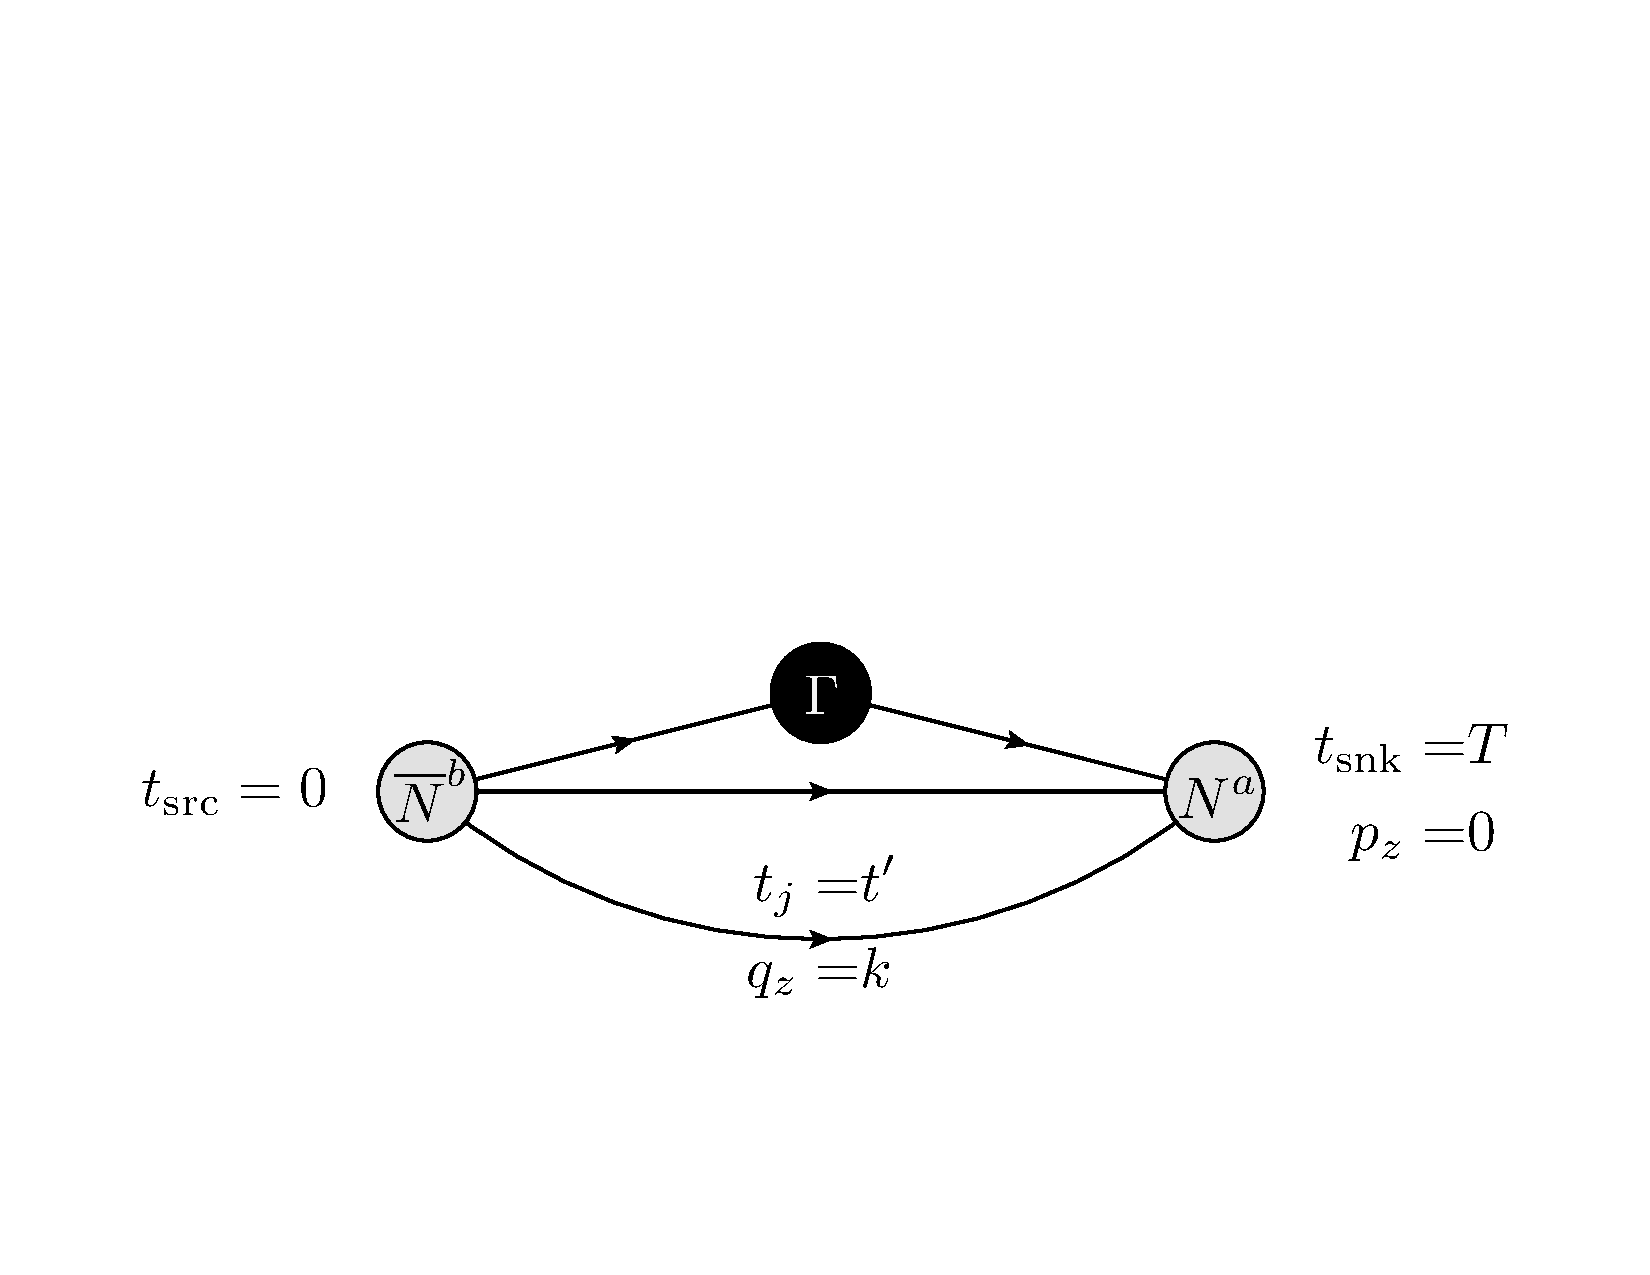
\includegraphics[width=\columnwidth]{./cropped_kinematics.pdf}
	\caption{Kinematics of the three-point correlator with baryon initial and final states. We work in the rest frame of the final hadron. The diagram for semi-leptonic decays of mesons involves only one spectator quark, but involves the same kinematics. {\color{red} Change $a$ and $b$ to say src and snk.}}
	\label{fig:3pt_kinematics}
\end{figure}
%{\color{red} Some more self-plagiarism.}
\subsubsection{Three-point correlation function}
We begin with a three-point correlation function with the sink state at
rest, and current insertion with three-momentum $k$, where, without
loss of generality we take $k$ to point
in the $z$-direction, as shown in
Fig.~\ref{fig:3pt_kinematics}, which we write as
\begin{align}
C^{\text{3pt}}(t, t^\prime) = \sum_{\vec{x},\vec{x}^\prime} \left<N^{\mathrm{snk}}_{t,\vec{x}}\Gamma_{t^\prime,\vec{x}^\prime} \overline{N}^{\mathrm{src}}_{0,\vec{0}}\right> e^{-ikz'},
\label{eq:3pt}
\end{align}
Here the current is at $(t', x', y', z')$, and the sink nucleon
operator is at $(t,x,y.z,)$; we use translation invariance to place the
source nucleon at the origin.
Since the sink has
zero three-momentum, and momentum is only inserted at the current,
momentum conservation implies that the three-momentum of the source
nucleon is $(0,0,k)$.
The operators $N^{\mathrm{src}}$ and
$N^{\mathrm{snk}}$ are the source and sink interpolation operators
respectively, allowing for different choices of the nucleon
interpolating operator~\cite{Basak:2005ir,Basak:2007kj} and operator
smearing profiles, and $\Gamma$ is a generic current
insertion such as the vector current discussed above.

The derivative of the three-point correlator with respect to $k^2$ follows,
\begin{align}
C^\prime_{\text{3pt}}(t, t^\prime)
=& \sum_{\vec{x},\vec{x}^\prime} \frac{-z'}{2k}\sin\left(k z'\right) \left<N^{\mathrm{snk}}_{t,\vec{x}}\Gamma_{t^\prime,\vec{x}^\prime} \overline{N}^{\mathrm{src}}_{0,\vec{0}}\right>, 
\label{eq:3ptmoment}
\end{align}
where in Eq.~(\ref{eq:3ptmoment}), the cosine component vanishes due to symmetry. In the limit of zero momentum, the $k^2 \rightarrow 0$ limit of the integrand is given by L'H\^opital's rule,
\begin{align}
\lim_{k^2 \rightarrow 0} C^\prime_{\text{3pt}}(t, t^\prime) = & \sum_{\vec{x},\vec{x}^\prime}\frac{-z^{\prime 2}}{2}\left<N^{\mathrm{snk}}_{t,\vec{x}}\Gamma_{t^\prime,\vec{x}^\prime} \overline{N}^{\mathrm{src}}_{0,\vec{0}}\right>.
\label{eq:3ptmoment0}
\end{align}

While it is tempting to think of Eq.~(\ref{eq:3ptmoment0}) as having an $x^{\prime 2}_z$ moment, it is clear from Eq.~(\ref{eq:3ptmoment}), that a single derivative contributes only a single factor of $x^{\prime}_z$. The second factor of $x^{\prime}_z$ only appears in the $k^2\rightarrow 0$ limit and should not be thought as a position-space moment resulting from a momentum-space derivative.

\subsubsection{Two-point correlation function}
Analogously, given a two-point correlator with three-momentum $k$ in the $z$-direction,
\begin{align}
C_{\text{2pt}}(t) = \sum_{\vec{x}} \left< N^{\mathrm{snk}}_{t,\vec{x}}\overline{N}^{\mathrm{src}}_{0,\vec{0}}\right> e^{-ikz},
\label{eq:2pt}
\end{align}
the derivative of the two-point correlator with respect to $k^2$ follows,
\begin{align}
C^\prime_{\text{2pt}}(t)
% \equiv & \frac{\partial}{\partial k^2} C_{\text{2pt}}(t),  \nonumber\\
= & \sum_{\vec{x}}\frac{-z}{2k} \sin\left(kz\right) \left<N^{\mathrm{snk}}_{t, \vec{x}}\overline{N}^{\mathrm{src}}_{0,\vec{0}} \right>.
\label{eq:2ptmoment}
\end{align}
 Analogous to the moment of the three-point correlator, the cosine contribution vanishes due to symmetry.  Consequently, in the zero-momentum limit,
\begin{align}
\lim_{k^2\rightarrow 0 } C^\prime_{\text{2pt}}(t) = \sum_{\vec{x}} \frac{-z^2}{2}\left<N^{\mathrm{snk}}_{t, \vec{x}}\overline{N}^{\mathrm{src}}_{0,\vec{0}} \right>.
\label{eq:2ptmoment0}
\end{align}
THus the construction of the moment of the two-point correlator is similar
to the moment of the three-point correlator, with the exception
the moment now depends on the final state position $z$ instead of
the current insertion position $z'$. In both cases, the
spatial dependence for all momenta are even, resulting in a
non-vanishing correlator under the Fourier transform, explicitly
circumventing the concern raised in Ref~\cite{Wilcox:2002zt}.  Given
the prior computational investment in generating the propagators and
sequential propagators, the generation of the moments of correlators
differs only during the computation of the Fourier transform, and therefore requires
negligible additional computing time to construct.


\subsection{Interpretation}
\subsubsection{Three-point correlation function}
In the rest frame of the final state hadron, the spectral decomposition of the three-point correlation function in Eq.~(\ref{eq:3pt}) is
\begin{align}
C_{\mathrm{3pt}}(t,t^\prime) = & \sum_{n,m}\frac{Z^{\dagger \mathrm{snk}}_m(0)\Gamma_{mn}(k^2)Z^{\mathrm{src}}_n(k^2)}{4E_m(0)E_n(k^2)}\nonumber \\
&\times e^{-E_m(0)(t-t^\prime)}e^{-E_n(k^2)t^\prime}. \label{eq:c3pt}
\end{align}
The time dependence involves the source-sink separation $t \equiv t^{\mathrm{snk}}-t^{\mathrm{src}}$ and the insertion-sink separation $t^{\prime}\equiv t^{\mathrm{ins}}-t^{\mathrm{src}}$. The parameters $E_n(k^2)$ infer the $n$-th state energy of the hadron with momentum $k^2$, $\Gamma_{mn}(k^2)$ infers the $n\rightarrow m$-th state matrix element, and $Z_{n(m)}^{\mathrm{src(snk)}}$ infers the overlap factor at the source and sink, which in general is different and depends on the interpolating operator and smearing profile used. On the lattice, the path integral is performed under a Wick rotation, yielding the exponential time dependence. At large time separations, the ground state signal exponentially dominates the correlation function.

Taking the $k^2$ derivative of Eq.~(\ref{eq:c3pt}) yields the spectral decomposition of the correlator generated by Eqs.~(\ref{eq:3ptmoment}, \ref{eq:3ptmoment0}),
\begin{align}
C^{\prime}_{\mathrm{3pt}}(t,t^\prime) = & \sum_{m,n}C^{mn}_{\mathrm{3pt}}(t,t^\prime)\left[\frac{\Gamma^\prime_{mn}(k^2)}{\Gamma_{mn}(k^2)}\right.\nonumber \\
&\left.+\frac{Z^{\prime\mathrm{src}}_n(k^2)}{Z^{\mathrm{src}}_n(k^2)}-\frac{1}{2E_n^2(k^2)}-\frac{t^\prime}{2E_n(k^2)}\right], \label{eq:c3ptm}
\end{align}
where $C^{mn}_{\mathrm{3pt}}$ is the $n\rightarrow m$-th state contribution of Eq.~(\ref{eq:c3pt}) and $\Gamma^\prime$ is the $k^2$ derivative of the matrix element $\Gamma$. Extracting $\Gamma^\prime$ is the main goal of this paper. An additional consequence is the dependence on $Z^{\prime\mathrm{src}}$, the $k^2$ derivative of the source overlap factor, which can be analogously extracted from the derivative of the two-point correlator. Here we note that in the rest-frame of the final hadron, only $Z^{\prime\mathrm{src}}$ survives, while any dependence on  $Z^{\prime\mathrm{snk}}$ explicitly vanishes, where the source and sink operators here apply to the three-point correlation function, and in general may be different from the operators used in the two-point correlator in the following discussion.

\subsubsection{Two-point correlation function}
The spectral decomposition of the two-point correlation function constructed from Eq.~(\ref{eq:2pt}) is,
\begin{align}
C_{\mathrm{2pt}}(t) = & \sum_m \frac{Z^{\dagger\mathrm{snk}}_m(k^2)Z^{\mathrm{src}}_m(k^2)}{2E_m(k^2)}e^{-E_m(k^2)t}
\label{eq:c2pt}
\end{align}
where on a given lattice, $t\equiv t^{\mathrm{snk}}-t^{\mathrm{src}}$ is the same source-sink separation $t$ in Eqs.~(\ref{eq:c3pt}, \ref{eq:c3ptm}). While in general, the source and sink operators may be different from the three-point correlation function, at least one of the operators has to be the same as the three-point source operator in order to disentangle $\Gamma^\prime$ from $Z^{\prime\mathrm{src}}$ from Eq.~(\ref{eq:c3ptm}).

Taking the $k^2$ derivative of Eq.~(\ref{eq:c2pt}) yields,
\begin{align}
C^\prime_{\mathrm{2pt}}(t) = & \sum_m C_{\mathrm{2pt}}^m(t)\left[\frac{Z^{\prime\dagger\mathrm{snk}}_m(k^2)}{Z^{\dagger\mathrm{snk}}_m(k^2)}+\frac{Z^{\prime\mathrm{src}}_m(k^2)}{Z^{\mathrm{src}}_m(k^2)}\right.\nonumber \\
&\left.-\frac{1}{2E_m^2(k^2)}-\frac{t}{2E_m(k^2)}\right],
\end{align}
where $Z^\prime$ is the $k^2$ derivative of the overlap factors. In particular, $Z^\prime = 0$ for point sources and sinks since a Dirac delta function provides equal support for all momenta.

\subsubsection{4-momentum derivatives}
The lattice correlation functions and the corresponding spectral decomposition is computed by directly taking the 3-momentum derivative. In general however, the radius of a hadron, or more generally the form factor, depends on the 4-momentum transfer squared $Q^2 = -q^2$ where
\begin{equation}
-q \equiv \begin{pmatrix} E_n(k^2)-M_m \\ 0 \\ 0 \\ k \end{pmatrix},
\end{equation}
which we again, assume that the final state hadron is at rest, such that $M_m = E_m(0)$. As a result, the $Q^2$ derivative of the matrix element is related to the $k^2$ derivative through the chain rule,
\begin{equation}
\frac{\partial}{\partial k^2}\Gamma_{mn} = \frac{\partial Q^2}{\partial k^2} \frac{\partial}{\partial Q^2} \Gamma_{mn} = \frac{M_m}{\sqrt{M_n^2+k^2}}\frac{\partial}{\partial Q^2} \Gamma_{mn},
\end{equation}
where $M_n$ and $M_m$ is respectively the rest mass of the initial and final state hadron.

\subsection{Reparameterization}
Dependence on the inverse of the matrix elements and overlap factors may lead to numerical instability especially when a large number of excited states are included in the fit ansatz. This is due to the fact that {\it{a priori}} the sign of the excited state parameters are unknown, and values close to zero may be sampled. In order to improve numerical stability, the following reparameterizations are suggested.

For the two- and three-point correlation function the factors of of $E$ are absorbed into the definition of $Z$ and $\Gamma$,
\begin{align}
C_{\textrm{2pt}}(t) = & \sum_m z^{\dagger\mathrm{snk}}_m(k^2) z^{\mathrm{src}}_m(k^2) e^{-E_m(k^2)t},\\
C_{\textrm{3pt}}(t,t^\prime) = & \sum_{m,n}z^{\dagger\mathrm{snk}}(0)g_{mn}(k^2)z_n^{\mathrm{src}}(k^2)\nonumber \\
&\times e^{-E_m(0)(t-t^\prime)}e^{-E_n(k^2)t^\prime},
\end{align}
such that
\begin{align}
z_n \equiv & \frac{Z_n(k^2)}{\sqrt{2E_n(k^2)}},\\
g_{mn} \equiv & \frac{\Gamma_{mn}(k^2)}{2\sqrt{E_m(0)E_n(k^2)}}.
\end{align}

Parameters from the derivative correlation function may be inferred using,
\begin{align}
C^\prime_{\mathrm{2pt}}(t) = & \sum_m C^m_{\mathrm{2pt}}(t)\left[z^{\prime\dagger\mathrm{snk}}_m(k^2)+z^{\prime\mathrm{src}}_m(k^2)\frac{}{}\right.\nonumber\\
&\left.-\frac{1}{2E_m^2(k^2)}-\frac{t}{2E_m(k^2)}\right],\\
C^\prime_{\mathrm{3pt}}(t,t^\prime)= & C_{\mathrm{3pt}}^{mn}(t,t^\prime)\left[g^\prime_{mn}(k^2)+z^{\prime\mathrm{src}}_n(k^2)\frac{}{}\right.\nonumber\\
&\left.-\frac{1}{2E_m^2(k^2)}-\frac{t^\prime}{2E_m(k^2)}\right],
\end{align}
where
\begin{align}
z^{\prime\mathrm{src(snk)}}_n\equiv & \frac{Z^{\prime\mathrm{src(snk)}}_n(k^2)}{z_n^{\mathrm{src(snk)}}(k^2)\sqrt{2E_n(k^2)}},\\
g^\prime_{mn} \equiv & \frac{\Gamma^\prime_{mn}}{2g_{mn}\sqrt{E_m(0)E_n(k^2)}}.
\end{align}

The Dirac radius contribution of Eq.~(\ref{eq:radius}), can therefore, be calculated directly from lattice QCD
\begin{align}
 -\frac{1}{6}\langle r_{\mathrm{Dirac}}^2 \rangle =& \left. \frac{\partial F_1(Q^2)}{\partial
	Q^2}\right|_{Q^2=0}\nonumber \\
=&g_{00} g^\prime_{00}.
\end{align}

\subsection{Valence finite volume correction}
The valence finite volume corrections results from 1) truncating the spatial moment at $z=L/2$, and applying the incorrect spatial moment between $[0,L/2]$ for periodic images coming from 2) $z\geq L$ and 3) $z \leq -L$. In this section we discuss how to correct for valence finite volume effects which arise from both contributions. In the following derivation, we make the assumption that past $L/2$, only the salient contribution comes from the ground state.

\begin{figure*}[t]{
		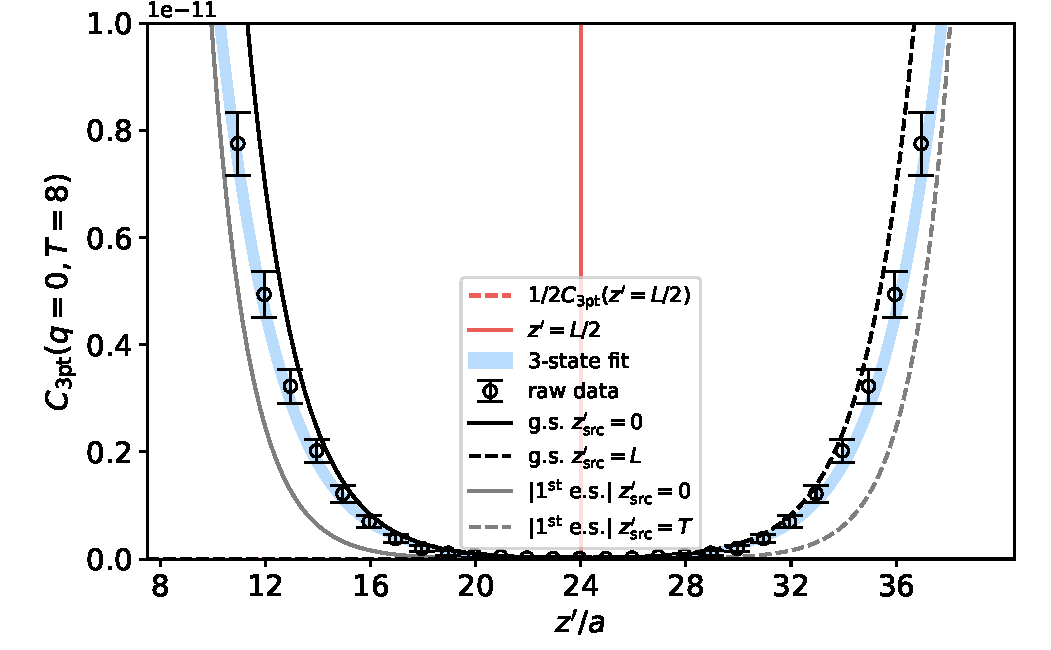
\includegraphics[width=0.49\textwidth]{figures/zcorr_3pt.pdf}
		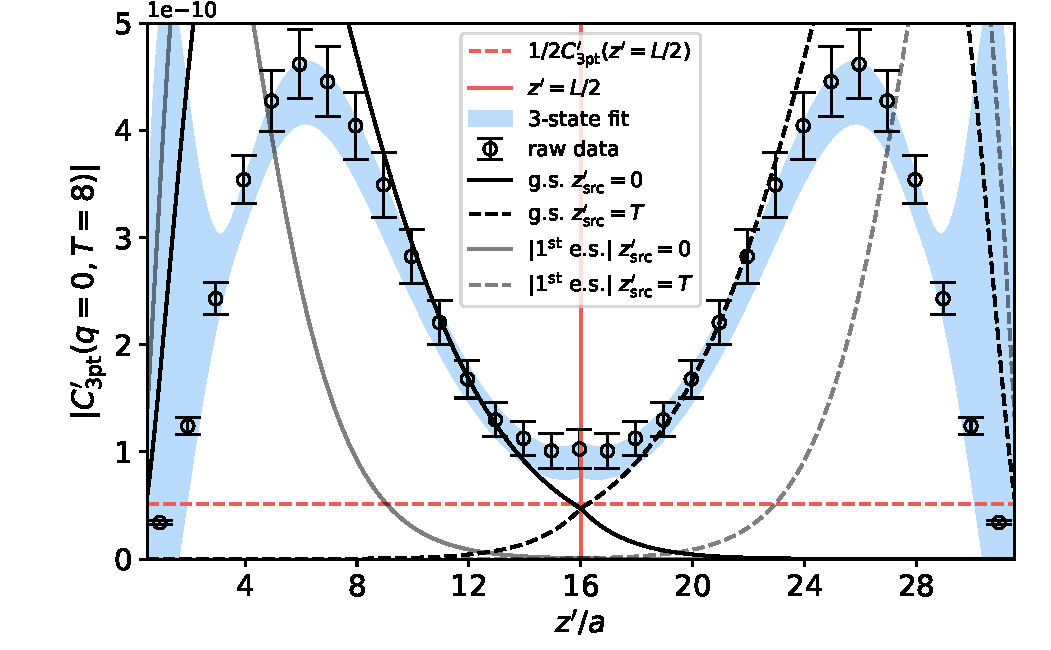
\includegraphics[width=0.49\textwidth]{figures/zcorr_d3pt.pdf}
		\caption{The left-hand plot shows the three-point
                  correlation function as a functions of the
                  current-insertion position $z'$, together with a
                  three-state fits to the form of eqn.~\ref{eq:3ptz}.
                  The lines denote the ground and first excited-state
                  contributions propagating from $z' = 0$ and $z'=L$,
                  respectively.  The right-hand plot shows the
                  corresponding data for the coordinated-weighted
                  correlation function.}
		\label{fig:finite_volume}
}\end{figure*}

Before discussing the volume corrections, we first discuss the various contributions to the three-point correlation function in the spatial direction. In Fig.~\ref{fig:finite_volume} (Left), we plot the correlator as a function of current insertion position $z^\prime$ after projecting to zero-momentum in $x^\prime$, $y^\prime$, and $t^\prime$. We then perform a 3-state fit from $z^\prime = [4,16]$ and extract the ground state and first excited-state parameters. Note that the correlator is symmetric by construction from averaging with the parity inverted counterpart, and in conjunction, a symmetric fit function is also employed defined as the following,
\begin{equation}
C(z^\prime) = \sum_n A_n\left(e^{-E_n z^\prime} + e^{-E_n(L-z^\prime)}\right).\label{eq:3ptz}
\end{equation} We observe that at $\sim 400$~MeV pion masses, the propagating scale in the spatial-direction for the three-point correlator is $\sim 820$~MeV, corresponding to the mass of the rho-meson ($m_\rho \sim 770$~MeV) {\color{red} what is the rho at 400 MeV?} with one unit of momentum ($\sim 120$~MeV) for a total energy of $\sim780$~MeV {\color{red} update if rho mass changes?}. This is consistent with expectation since the vector current yields a vector-meson propagating state, and the temporal direction has anti-periodic boundary conditions with length $T=96$. Additionally, we observe that beyond $L/2$, the correlation function is dominated by the ground state.

In Fig.~\ref{fig:finite_volume} (Right), we take the results from Fig.~\ref{fig:finite_volume} (Left) and construct the zero-momentum moment correlation function. As expected, the spatial moment pushes the dominant contribution of the correlation function to larger values of $z^\prime$ (maximally around $z^\prime \sim 7$ instead of at zero). Additionally, since the spatial moment is itself not periodic and truncated at $z^\prime = L/2$, the moment correlation function deviates from Eq.~(\ref{eq:3ptmoment0}). We observe again however, that only the ground-state needs to be considered, since the first-excited state has insignificant contribution for $z^\prime \geq L/2$.

The positive-correction to truncating the spatial moment at $L/2$ is given as follows.
\begin{align}
\left.\delta^n_{1}\right|_{k\neq 0}= & 2\int_{L/2}^{\infty} \frac{-iA_n}{2k} z(-i \sin(kz))e^{-E_n z} dz \label{eq:dfv_1.1}\\
=& \frac{A_n e^{-E_n L/2}}{2(E_n^2+k^2)^2}(-1)^m\left[E_n^2L+k^2L+4E_n\right] \label{eq:dfv_1.2}\\
\lim_{k\rightarrow 0}\delta^n_{1} =& -A_n\left(\frac{L^2}{4E_n}+\frac{L}{E_n^2}+\frac{2}{E_n^3}\right)e^{-E_n L/2}. \label{eq:dfv_1.0}
\end{align}
The factor of 2 in Eq.~(\ref{eq:dfv_1.1}) arises from performing a symmetric integral around the origin, $E_n$ is the $n$-th state energy, $A_n$ is the $n$-th state coefficient of the correlation function, and $k=\frac{2m\pi}{L}$ which simplifies $\cos(kL/2) = (-1)^m$. Taking the zero-momentum limit requires keeping the $\sin({kL/2})$ contribution of Eq.~(\ref{eq:dfv_1.2}), which otherwise vanishes at non-zero momentum from symmetry.

The negative-correction from applying the spatial moment to periodic images from $z^\prime \geq L$ is derived below. 
\begin{align}
\left.\delta^n_{2}\right|_{k\neq 0} =& 2\int_0^{L/2} \frac{-iA_n}{2k}z(-i\sin(kz)) \sum_{s=1}^\infty e^{E_0(z-sL)} dz \label{eq:dfv_2.1}\\
= & \frac{A_n e^{-E_n L}}{1-e^{-E_n L}}\frac{1}{2(E_n^2+k^2)^2}\nonumber\\
&\times\left[(-1)^m e^{E_n L/2}(E_n^2L+k^2L-4E_n) + 4E_n\right]\label{eq:dfv_2.2}\\
\lim_{k\rightarrow 0}\delta^n_2= & \frac{A_n e^{-E_n L}}{1-e^{-E_n L}}\nonumber\\
&\times\left[e^{E_n L/2} \left( -\frac{L^2}{4E_n} + \frac{L}{E_n^2} -\frac{2}{E_n^3} \right) + \frac{2}{E_n^3}\right].
\label{eq:dfv_2.0}
\end{align}

Finally, the negative-correction from applying the spatial moment to periodic images from $z^\prime \leq -L$ is,
\begin{align}
\left.\delta^n_{3}\right|_{k\neq 0}= & 2\int_{0}^{L/2}  \frac{-iA_n}{2k} z (-i\sin(kz)) \sum_{s=1}^\infty e^{-E_n(z+sL)} dz \label{eq:dfv_3.1}\\
=&\frac{A_n e^{-E_n L}}{1-e^{-E_n L}}\frac{1}{2(E_n^2+k^2)^2}\nonumber\\
&\times\left[(-1)^m e^{-E_n L/2}(E_n^2L+k^2L+4E_n) - 4E_n\right]\\
\lim_{k\rightarrow 0} \delta^n_3= & \frac{A_n e^{-E_n L}}{1-e^{-E_n L}}\nonumber\\
&\times \left[ e^{-E_n L/2}\left(\frac{L^2}{4E_n}+\frac{L}{E_n^2}+\frac{2}{E_n^3}\right)-\frac{2}{E_n^3}\right].
\label{eq:dfv_3.0}
\end{align}

{\color{red} non-zero momentum FV correction needs to be check. I'm pretty sure there's an error some where. The zero-momentum should be correct though.} The complete valence finite volume correction is
\begin{equation}
\delta_{\mathrm{valence}} = \sum_{n=0}^\infty \delta^n_1 - \delta^n_2 - \delta^n_3,
\label{eq:total_vfv}
\end{equation}
However, in practice Fig.~\ref{fig:finite_volume} suggests that one may only need to consider the ground-state contribution from $z^\prime_{\mathrm{src}}=\{0, L\}$. Specifically for the small-volume (l3296) $T=8$ moment correlator, after substituting $A_0$ and $E_0$ into Eq.~(\ref{eq:total_vfv}), we estimate the valence finite volume effect to be a $6.0\pm 1.2$\% correction to the correlation function summed over $z^\prime$. Under the assumption that excited-state are insignificant, this correction is independent of source-sink separation time within the quoted uncertainty. Fig.~\ref{fig:fv_relerr} shows the size of the relative volume correction as a function of the spatial length $L$ and ground state energy $E_0$.

\begin{figure}[t]{
		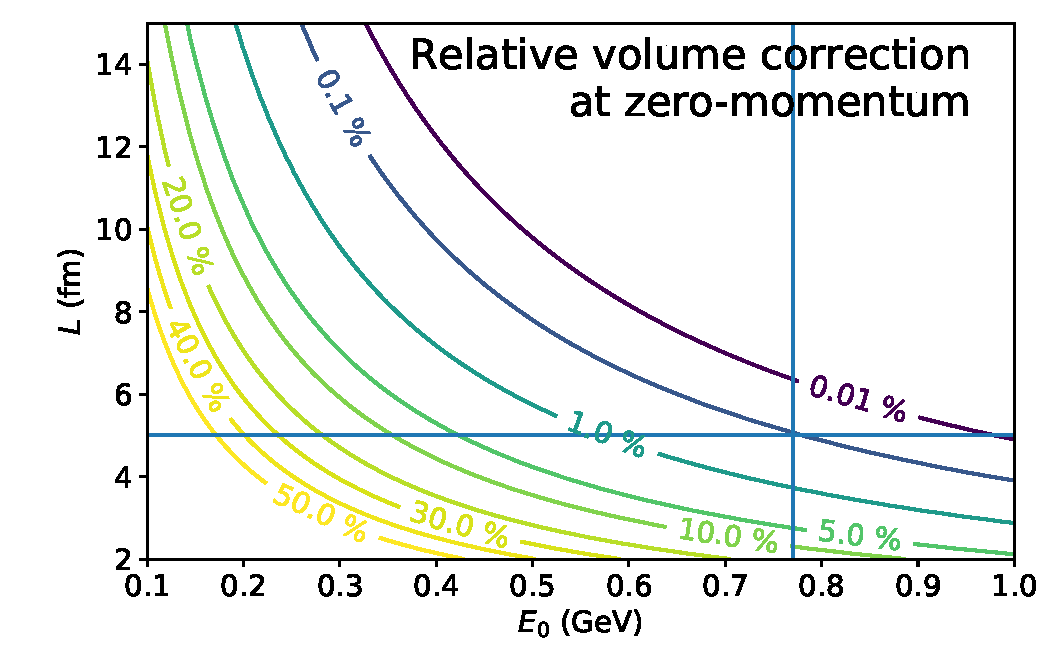
\includegraphics[width=0.49\textwidth]{figures/fv_relerr_0mom.pdf}
		\caption{(Left) blah blah..}
		\label{fig:fv_relerr}
}\end{figure}

Because the volume correction relies on extracting $A_0$ and $E_0$ after 3-momentum projection, the volume corrected three-point correlation function should be analyzed using the summation method. However, the data set of this preliminary study only has two source-sink separations and precludes such an option. In the example calculation discussed in Sec.~\ref{sec:results}, we demonstrate the efficacy of this method without considering the volume correction.

Finally, the two-point moment correlation function has analogous volume corrections, propagating with the mass of the final state hadron with one unit of momentum ($\sim 1.47$~GeV), which in this study corresponds to the nucleon ($m_N \sim 1.32$~GeV). As a result, the volume corrections are exponentially damped compared to the three-point moment correlation functions, and only contribute to a correction of $0.070(5)$\% to the small volume (l3296) calculation. It is important to point out that while the volume effects are small for the two-point correlation function, it can not be corrected by Eq.~(\ref{eq:total_vfv}) via the summation method. {\color{red} Discuss ideas to circumvent this? or just leave it as is.}


\section{Dirac radius of the nucleon}\label{sec:results}

\subsection{Computational Details}
To demonstrate the efficacy of this approach, we perform the
calculation on the Jefferson Lab isotropic clover lattices, with two light
(up/down) quark flavors, and a strange quark, that is fixed to its
physical value, and at two different volumes.  Since an important aim
of this paper is to investigate the dependence of the results on the
spatial volume of the box in which the calculation is performed, we
work at relatively coarse lattice spacing of approximately 0.12fm; in contrast to the
preliminary results presented in ref.~\cite{Bouchard:2016gmc}, these
ensembles have larger spatial volume, and are not replicated along the $z$-direction.  Properties of the ensembles are summarized in Table~\ref{tab:cfg}.
\begin{table}
  \begin{tabular}{cccccccc}
  	\hline\hline
    Label & Size & $\beta$ & $a$[fm] & $m_\pi$[MeV] & $m_\pi L$ & $N_{\rm cfg}$ & $N_{\rm src}$\\
    \hline
    l3296 & $32^3 \times 96$ & 6.1 & 0.12 & 400 & 7.7 & 196 & 2\\
    l4896 & $48^3 \times 96$ & 6.1 & 0.12 & 400 & 11.5 & 98 & 2\\
    \hline\hline
  \end{tabular}
  \caption{The details of the ensembles used in the calculation, denoted by the labels in the first column.  The
    lattice spacing is obtained using $\omega_0$ to set the scale,
    while the final column lists the number of time sources used for
    the two-point and three-point functions on each
    configuration.\label{tab:cfg}}
\end{table}


The three-point correlation functions are constructed using a \textit{sequential propagator} with sink-locations at $T=[8,10]$, and projected to $k^\prime=[0,2\pi/L]$ momentum at the interaction, and zero-momentum at the sink. The two-point correlation function is projected to $k=[0,2\pi/L]$ momentum at the sink. While not considered in this study, this method can also be applied to the Breit frame.

\subsection{Analysis strategy}
For the following analysis, parametric inference is performed under the Bayesian framework and implemented by the Python library \texttt{lsqfit}~\cite{lsqfit-9.3}. The posterior distributions are extracted from a \textit{chained fit} to $C_{\mathrm{2pt}}(t)$, $C^\prime_{\mathrm{2pt}}(t)$, $C_{\mathrm{3pt}}(t,t^\prime)$, and $C^\prime_{\mathrm{3pt}}(t,t^\prime)$ for $k^{(\prime)}=[0,2\pi/L]$. A chained fit sequentially minimizes the loss function against each correlation function while preserving the covariance between all data and posterior distributions. Due to having relatively low statistics, a chained fit is employed to limit the number of degrees-of-freedom in each step of the chain, and avoids systematic errors that arise from inverting an ill-conditioned covariance matrix. Robustness of the fit is demonstrated by performing a sensitivity analysis under varying fit regions for all 8 correlation functions. Additionally, we check that the ground state energy and the overlap factors satisfy the dispersion relation over different momenta. We include only the first excited state in fit ansatz to avoid an under-constrained fit against three-point correlation functions with two source-sink separations times.

\subsection{Analysis details}
\subsubsection{Prior selection}
The ground state priors $(\tilde{E}_0, \tilde{z}_0, \tilde{z}^\prime_0, \tilde{g}_{00}, \tilde{g}^\prime_{00})$ are loosely constrained through visual inspection of the respective plateau values shown in Fig.~\ref{fig:effective_mass} and Fig.~\ref{fig:effective} obtained from plotting the \textit{effective mass} and other similar quantities. The prior widths are orders of magnitude wider than the resulting ground state posterior distributions for all parameters.

\begin{figure}[t]{
	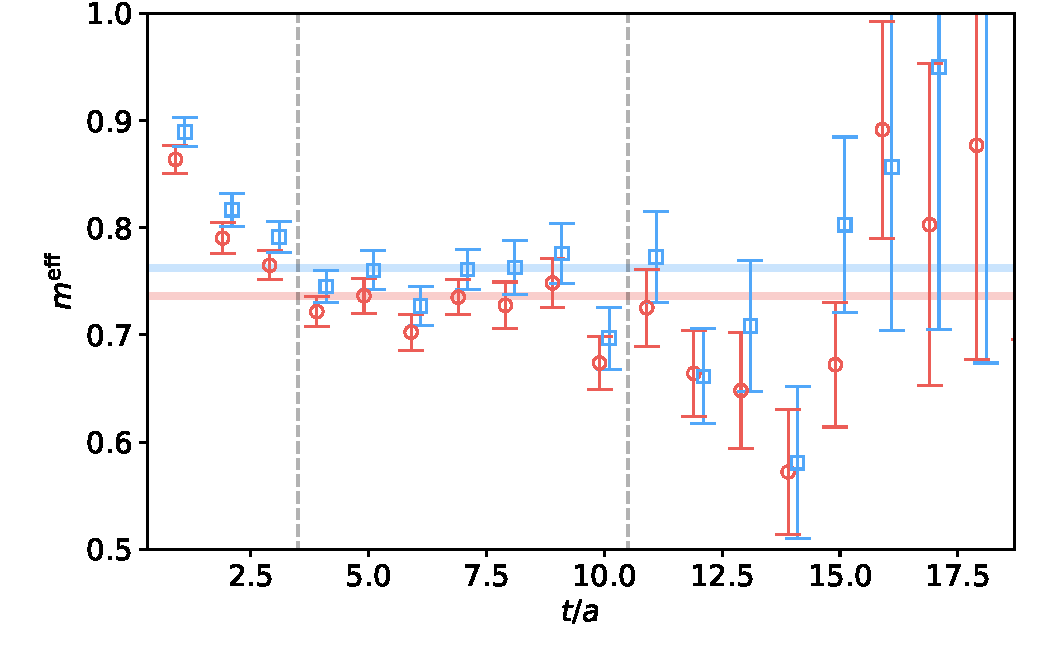
\includegraphics[width=0.49\textwidth]{figures/3296_meff.pdf}
	\caption{Effective mass.}
	\label{fig:effective_mass}
}\end{figure}

The excited-state energy is parameterized as a log-normal splitting with the median at the two-pion splitting with the one-pion splitting within the 68\% credible interval. The excited-state overlap factor is set to $\tilde{z}_1\sim \mathcal{N}(0,\langle \tilde{z}_0\rangle/2)$, reflecting the fact that we expect the magnitude to be half the ground state mean value due to operator smearing, but are agnostic about the sign. The excited-state slope of the overlap factor is set to the same distribution as the ground state, since we expect the slope to be constant up to discretization corrections as required by the dispersion relation. The excited-state vector charges and radii are set to $\tilde{g}^{(\prime)}_{nm}\sim \mathcal{N}(0,\langle \tilde{g}^{(\prime)}_{00}\rangle)$ with similar reasoning as $\tilde{z}_1$. 

\subsubsection{Fit region and sensitivity analysis}

\begin{figure}[b]{
		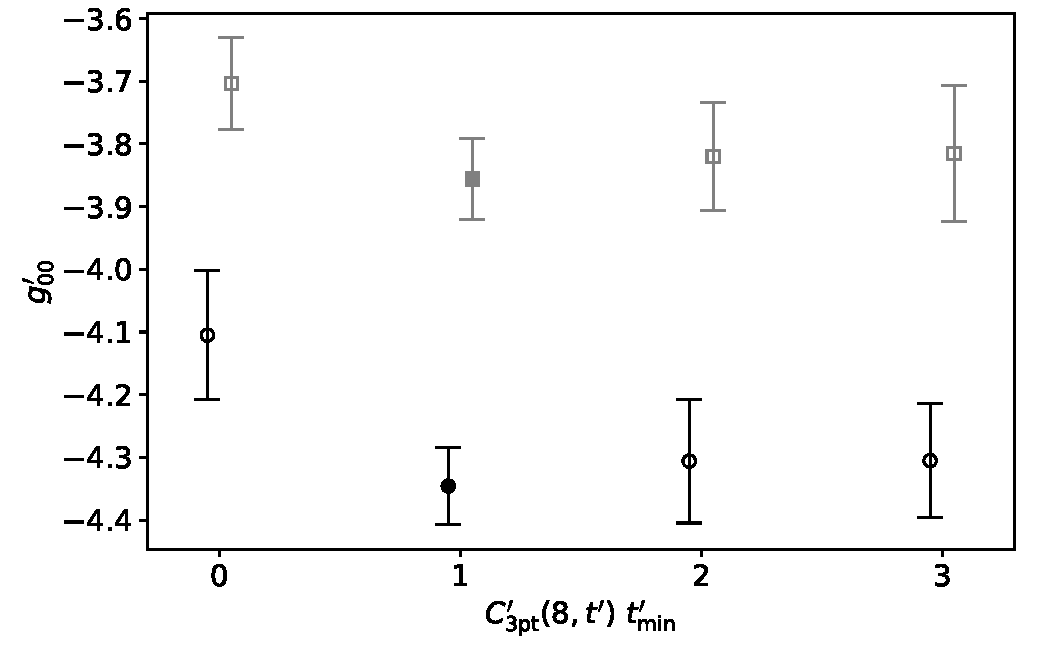
\includegraphics[width=0.49\textwidth]{figures/3296_dgV8_dgV.pdf}
		%\includegraphics[width=0.49\textwidth]{figures/3296_dgV8_tmax_dgV.pdf}
		\caption{Stability plot.}
		\label{fig:stability_main}
}\end{figure}

The robustness of the final results are demonstrated by observing stability of the ground state under varying the fit region across all eight correlation functions. Fig.~\ref{fig:stability_main} shows that the ground state radius is stable when fitting over different values of $t^\prime_{\mathrm{min}}$ and $t^\prime_{\mathrm{max}}$. We remind the reader that $t^\prime$ denotes the current insertion time, and a complete analysis should also include a study of stability under varying the source-sink separation time $t$. The complete study of the fit region, to the extent permitted by the data, is shown in Sec.~\ref{Appendix:small_volume_stability}.

In Fig.~\ref{fig:effective_mass} and Fig.~\ref{fig:effective}, the data between the vertical gray lines are included in the analysis of the preferred fit. We observe that the resulting ground-state posterior distributions lie on top of the expected value suggested by the effective mass and analogous plots. The posterior distribution is observed to be consistently more precise than what the individual correlation functions suggests because a correlated analysis is performed across all data sets.

\subsubsection{Finite volume effects}
{\color{red} Need 4896 data...}

\subsection{Results}
We present the first results from applying the spatial moments method for extracting directly from LQCD, the slope of the isovector vector form factor. In Fig.~\ref{fig:radius}, the values of $Z_0$ and $g_V$ at zero (black) and 350~MeV (red) momentum ($k=[0, 2\pi/L]$) are extracted from the lattice calculation. Additionally, the slope of the dashed lines are directly extracted from the same lattice calculation from the analysis of the correlation function with the spatial moment.

{\color{red} Work out disc. correction to dispersion relation (Wilson should still be asq). Say if Z follows dispersion relation.}


Following this analysis, we quote the value of the isovector Dirac radius of the nucleon to be
\begin{equation}
\left( r_1 \right) ^{u-d} = 0.1753(64)\ \mathrm{fm}
\end{equation}
on the $a\sim 0.11$~fm and $m_\pi \sim 400$~MeV isoclover lattice with a 4\% statistical uncertainty.

\begin{figure*}[t]{
		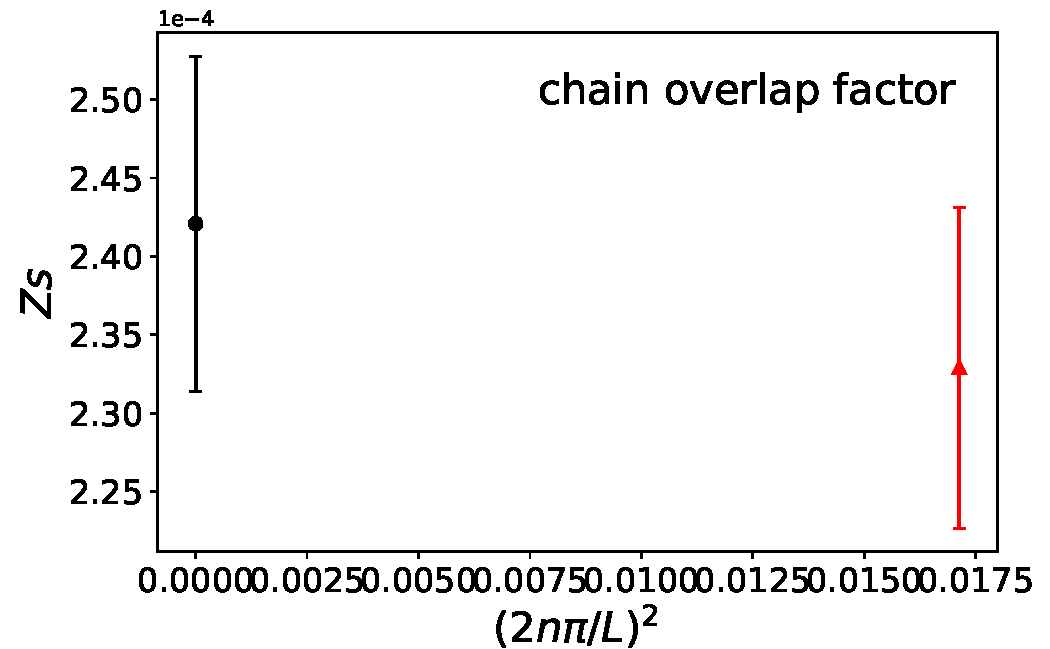
\includegraphics[width=0.49\textwidth]{figures/Zs_chain.pdf}
		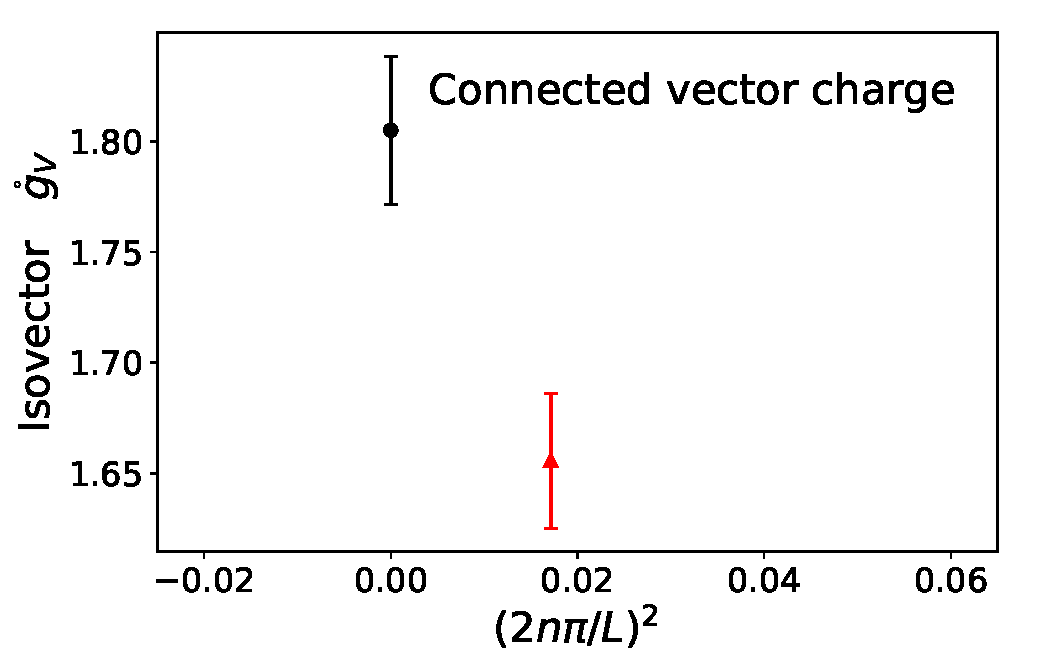
\includegraphics[width=0.49\textwidth]{figures/gV_chain.pdf}
		\caption{(Left) Stability plot and (Right) $Q$-value for the matrix element derivative under varying $t_{\mathrm{min}}$ of the two-point correlation function, and $n$-states. The preferred fit is shown by the solid green points.}
		\label{fig:radius}
}\end{figure*}

\section{Conclusions and outlook}
This is a great paper. Please publish. Thanks.


%%%%%%%%%%%%%%%%%%%%%%%%%%%%%%
\bibliography{pcr_bib}
%%%%%%%%%%%%%%%%%%%%%%%%%%%%%%

%\begin{comment}
\appendix

\clearpage
\newpage
\onecolumngrid

\section{Small volume effective mass and related plots}
\begin{figure*}[h]{
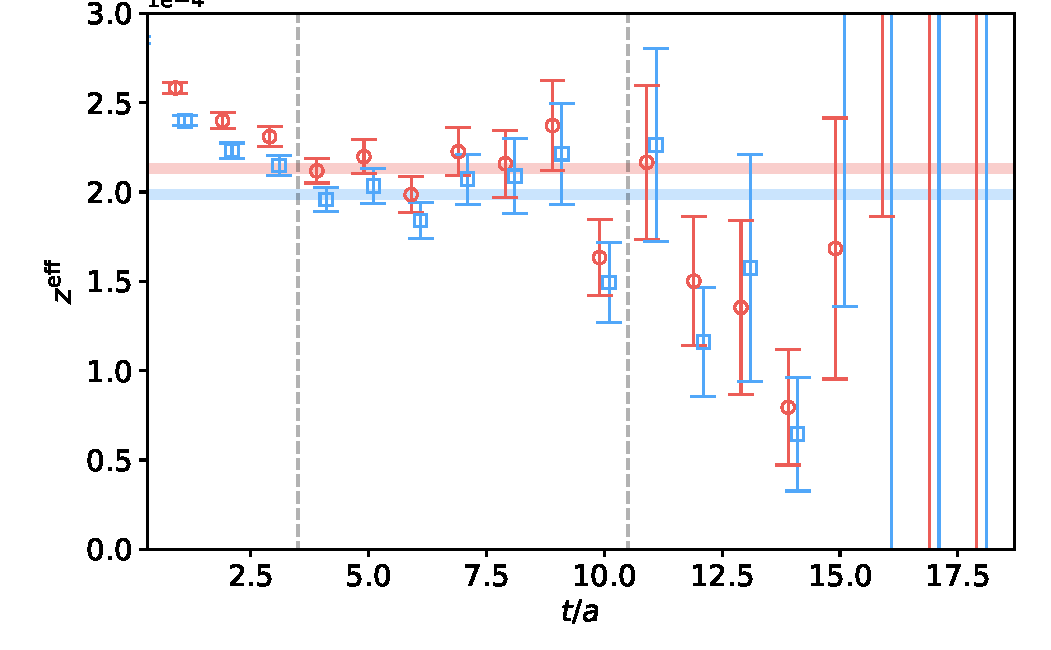
\includegraphics[width=0.49\textwidth]{figures/3296_zeff.pdf}
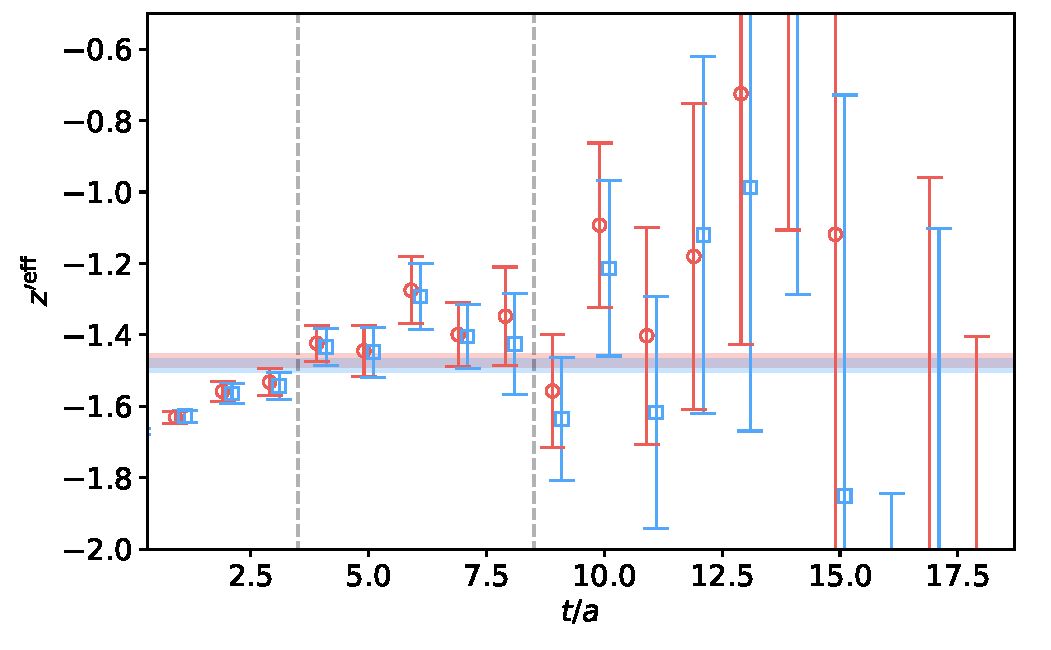
\includegraphics[width=0.49\textwidth]{figures/3296_dzeff.pdf}
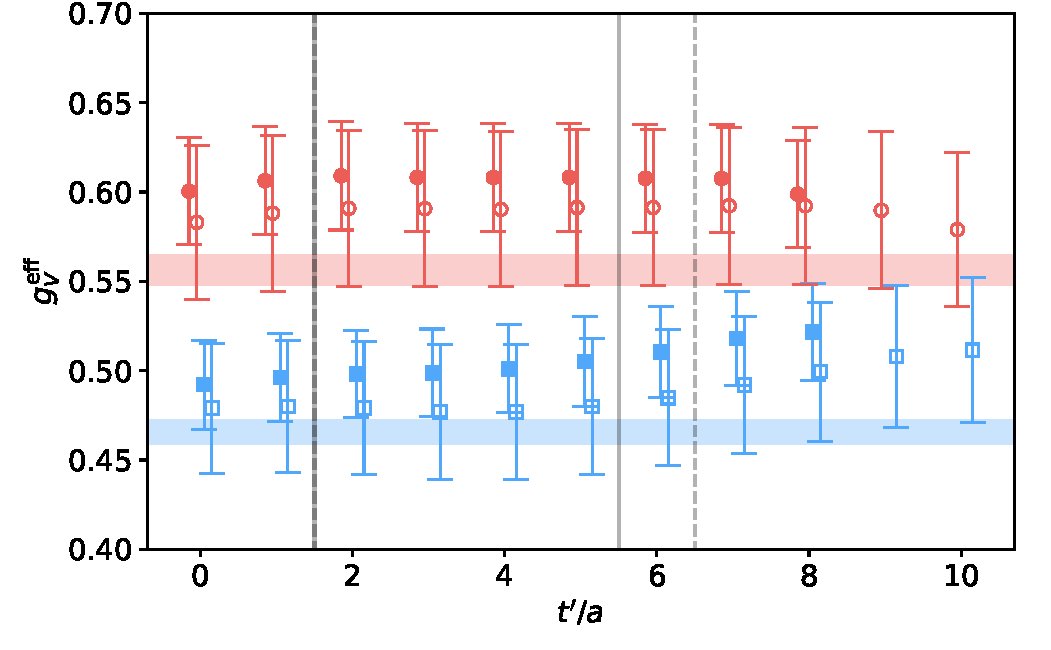
\includegraphics[width=0.49\textwidth]{figures/3296_gVeff.pdf}
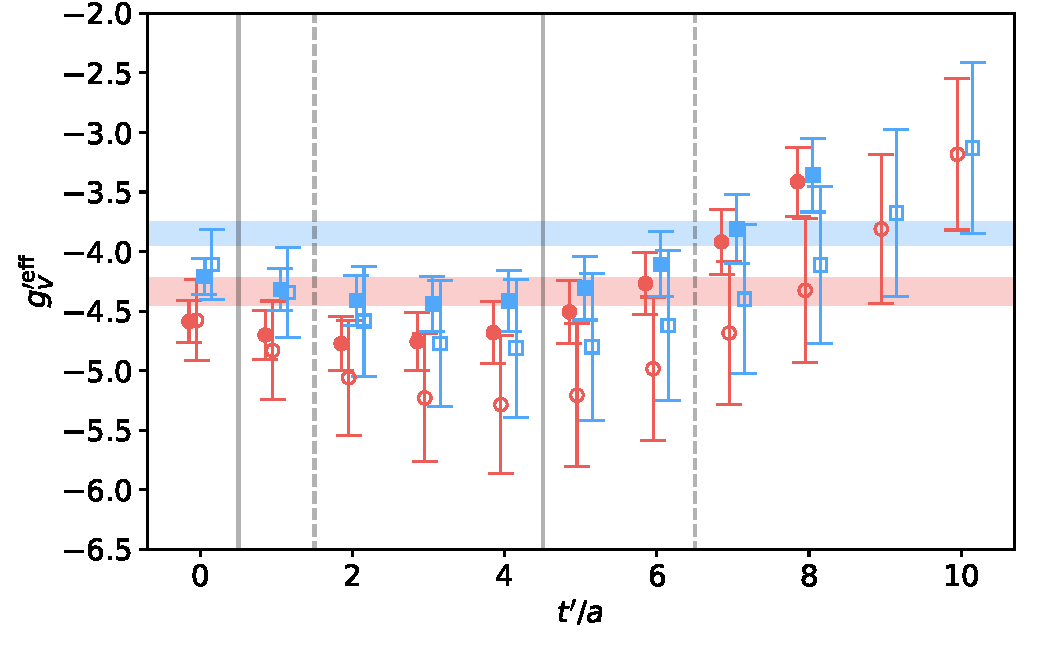
\includegraphics[width=0.49\textwidth]{figures/3296_dgVeff.pdf}
\caption{(Left) Stability plot and (Right) $Q$-value for the matrix element derivative under varying $t_{\mathrm{min}}$ of the two-point correlation function, and $n$-states. The preferred fit is shown by the solid green points.}
\label{fig:effective}
}\end{figure*}

\clearpage
\newpage
\section{Small volume $t_{\mathrm{max}}$ correlator stability plots}
\label{Appendix:small_volume_stability}
\begin{figure*}[h]{
		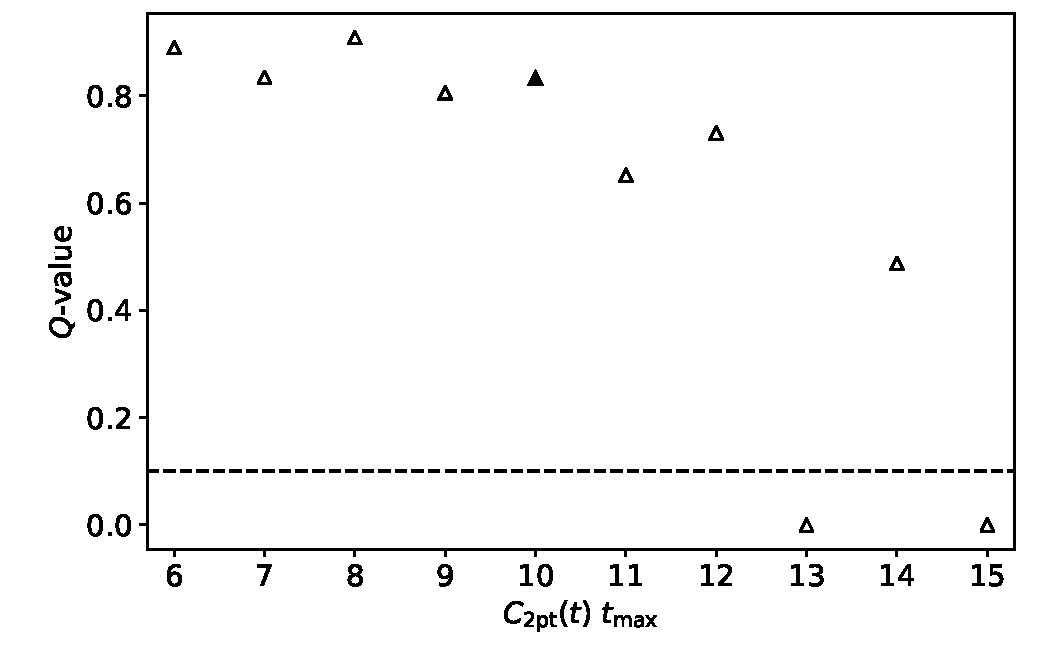
\includegraphics[width=0.49\textwidth]{plots/figures/3296_2pt_tmax_Q.pdf}
		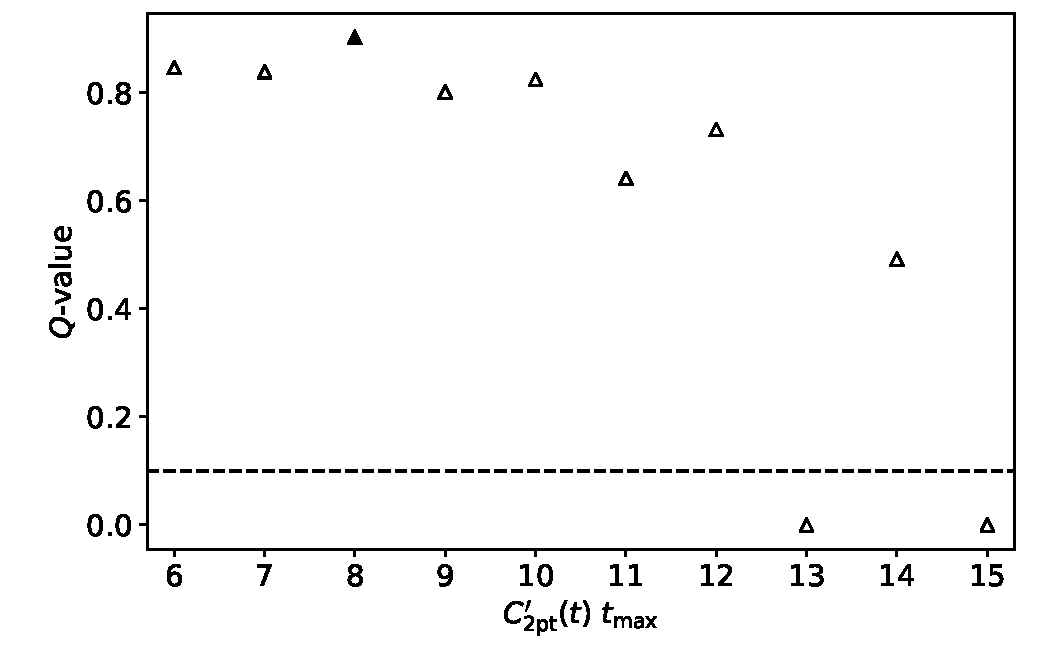
\includegraphics[width=0.49\textwidth]{plots/figures/3296_d2pt_tmax_Q.pdf}
		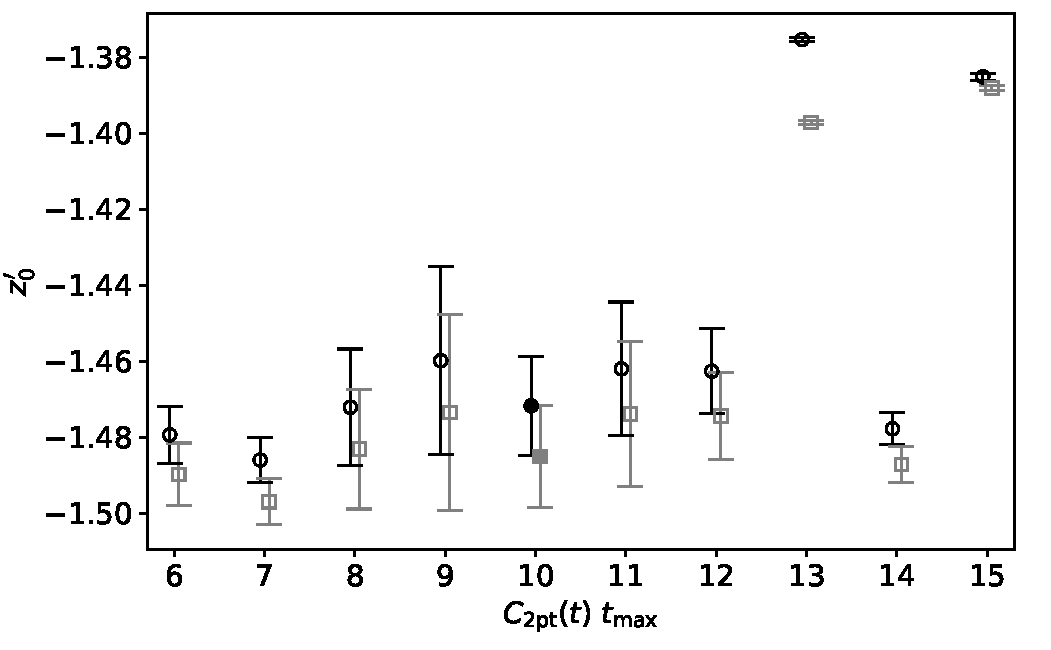
\includegraphics[width=0.49\textwidth]{plots/figures/3296_2pt_tmax_dZ0.pdf}
		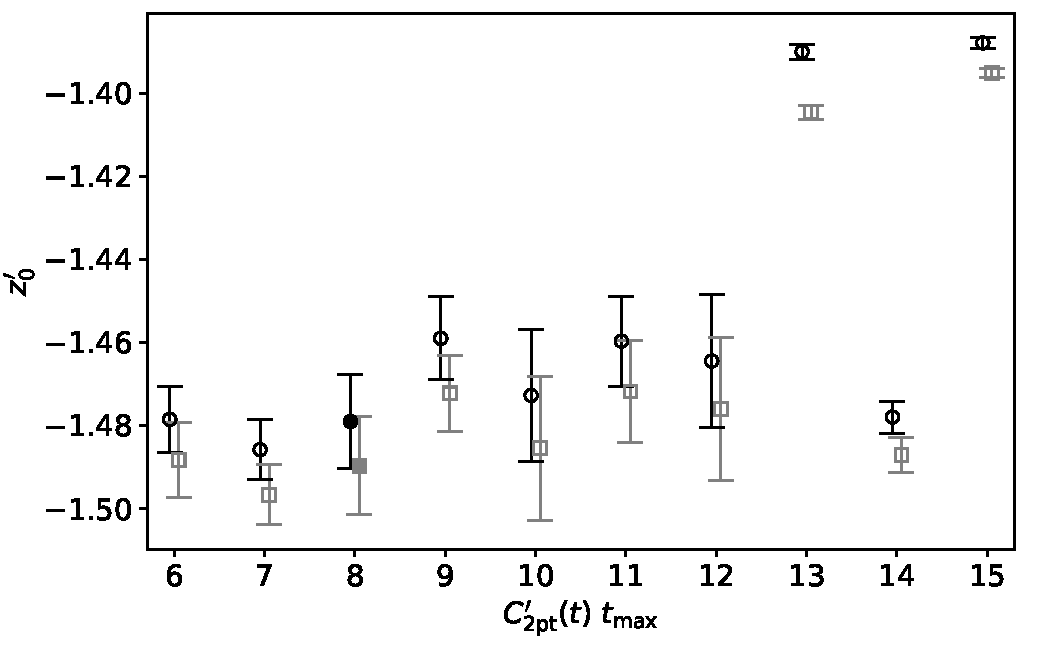
\includegraphics[width=0.49\textwidth]{plots/figures/3296_d2pt_tmax_dZ0.pdf}
		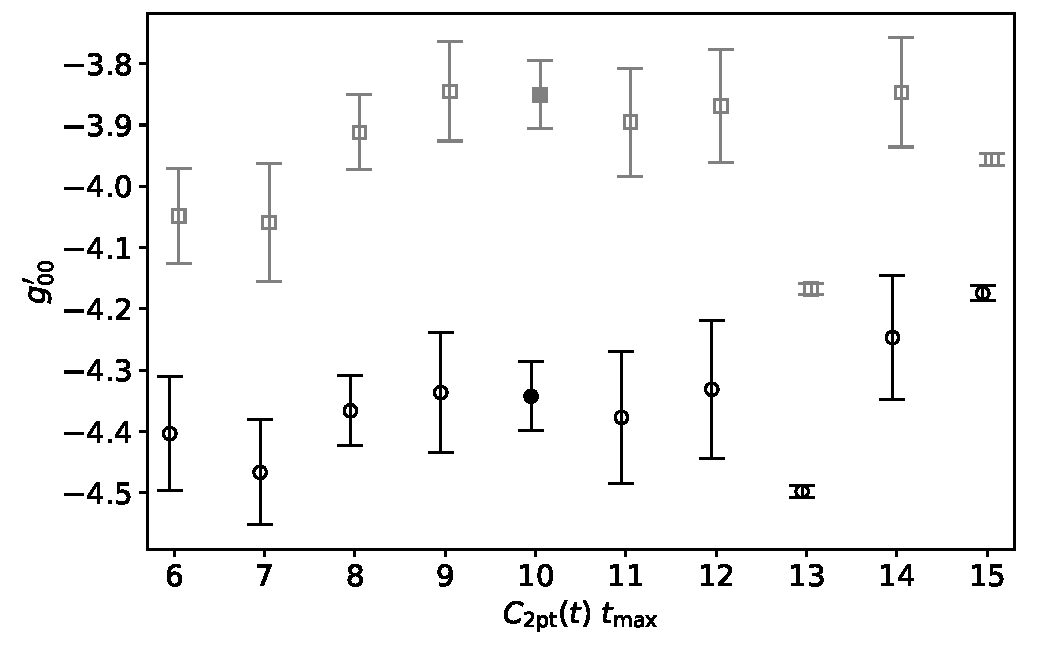
\includegraphics[width=0.49\textwidth]{plots/figures/3296_2pt_tmax_dgV.pdf}
		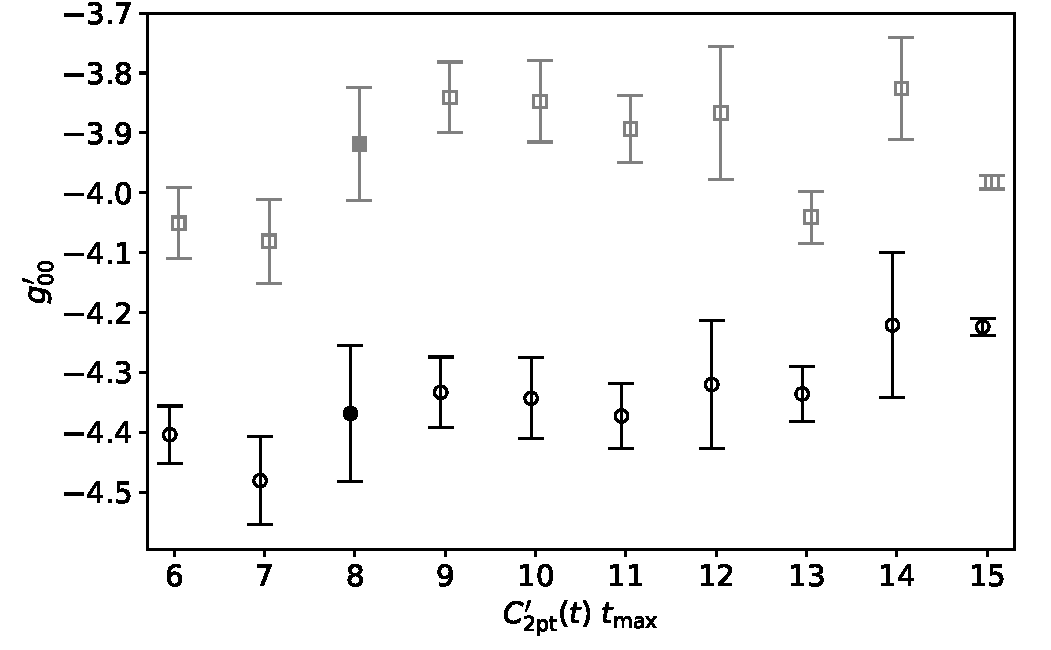
\includegraphics[width=0.49\textwidth]{plots/figures/3296_d2pt_tmax_dgV.pdf}
		\caption{Fit sensitivity to variations of $C_{\mathrm{2pt}}(t)$ and $C^\prime_{\mathrm{2pt}}(t)$ fit regions. Shown here are the $t_{\mathrm{max}}$ and $n$-state stability plots for the $Q$-value (top row), $z^\prime_0$ (middle row) and $g^\prime_{00}$ (bottom row). The colors indicate fits with $n$-state=1 (red), 2 (green), 3 (blue), and 4 (purple). The different momenta are given by k=0 (circle), and k=$2\pi/L$ (square). The preferred fit is denoted by the solid symbol. The dashed line is set to $Q=0.1$. The $t_{\mathrm{max}}$ values are integer-valued and staggered for visual clarity.}
		\label{fig:stability_c2pt}
}\end{figure*}

\newpage
\begin{figure*}[h]{
		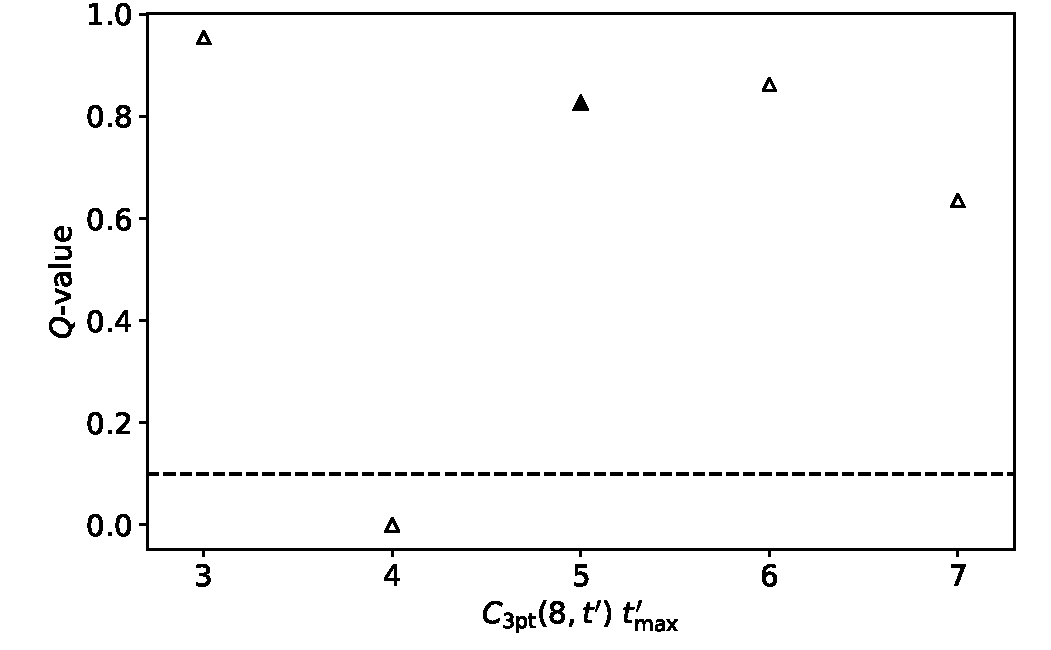
\includegraphics[width=0.49\textwidth]{plots/figures/3296_gV8_tmax_Q.pdf}
		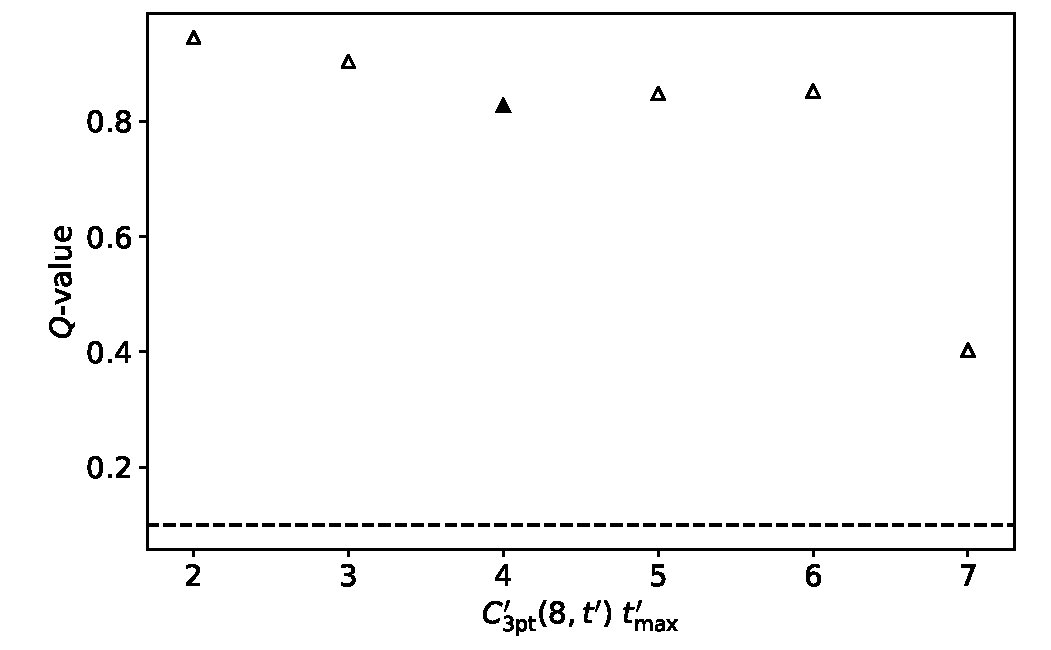
\includegraphics[width=0.49\textwidth]{plots/figures/3296_dgV8_tmax_Q.pdf}
		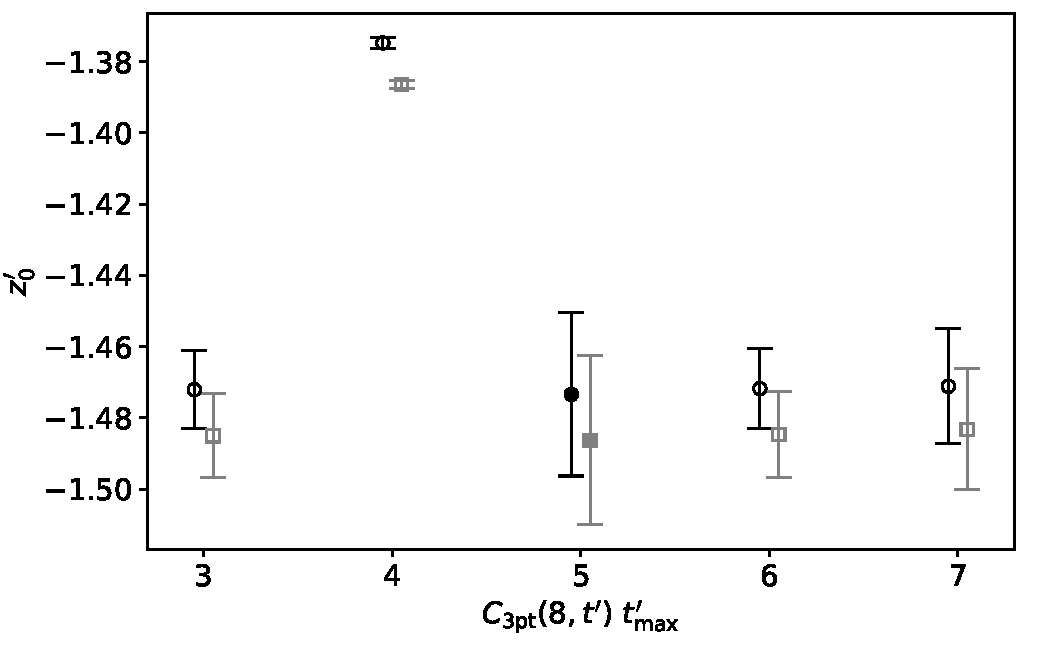
\includegraphics[width=0.49\textwidth]{plots/figures/3296_gV8_tmax_dZ0.pdf}
		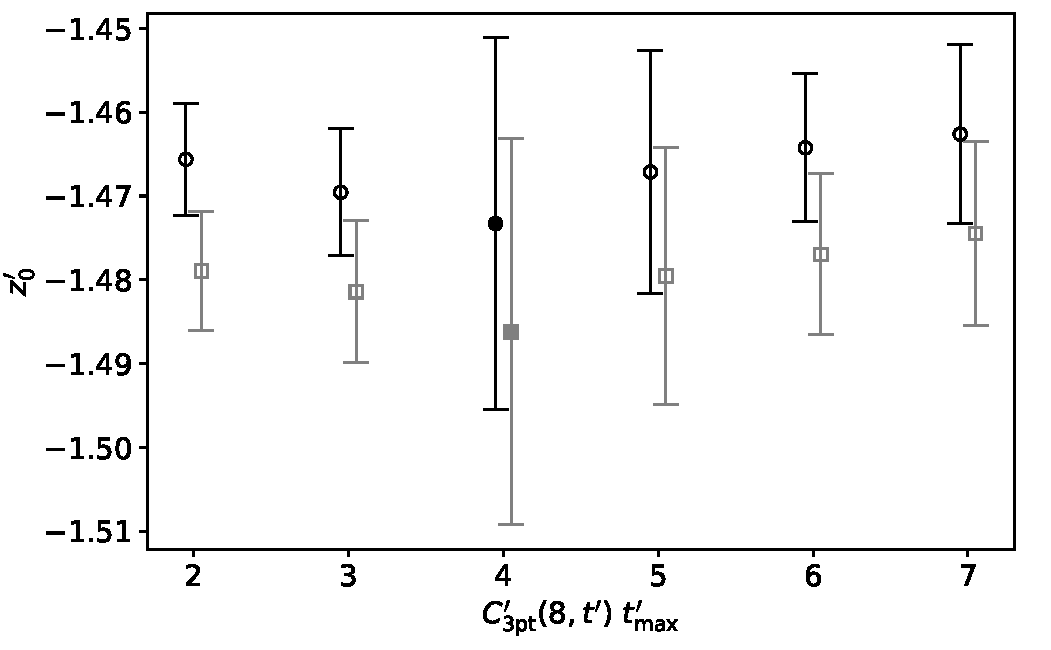
\includegraphics[width=0.49\textwidth]{plots/figures/3296_dgV8_tmax_dZ0.pdf}
		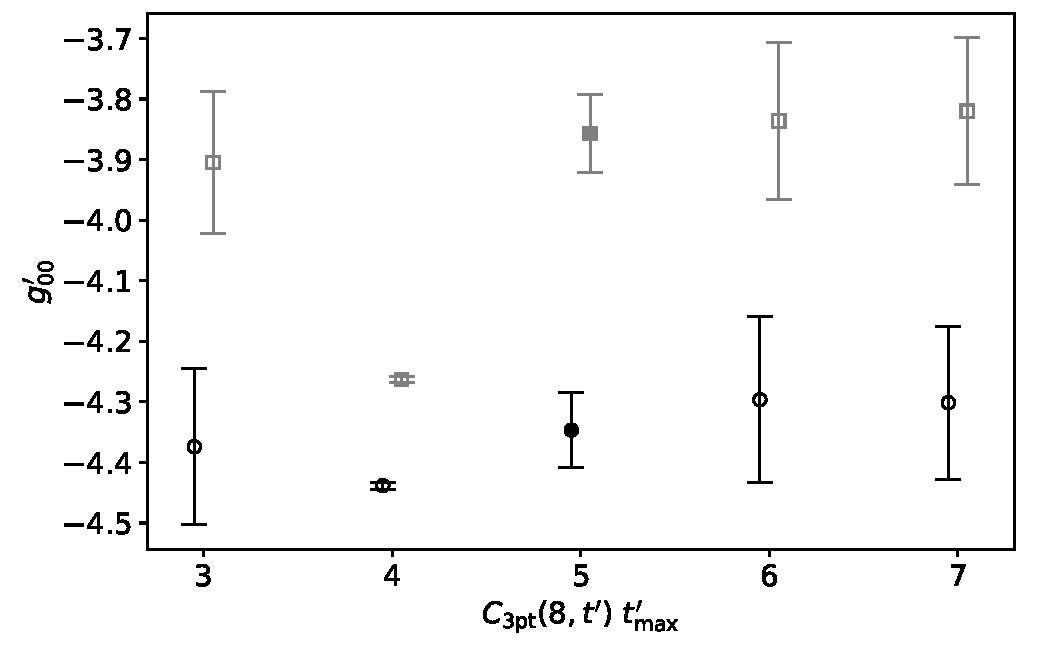
\includegraphics[width=0.49\textwidth]{plots/figures/3296_gV8_tmax_dgV.pdf}
		\includegraphics[width=0.49\textwidth]{plots/figures/3296_dgV8_tmax_dgV.pdf}
		\caption{
			Fit sensitivity to variations of $C_{\mathrm{3pt}}(8,t^\prime)$ and $C^\prime_{\mathrm{3pt}}(8,t^\prime)$ fit regions. For $C_{\mathrm{3pt}}$, the data is removed symmetrically around the mid-point. Analogous to Fig.~\ref{fig:stability_c2pt}.}
		\label{fig:stability_c3pt8}
}\end{figure*}

\newpage
\begin{figure*}[h]{
		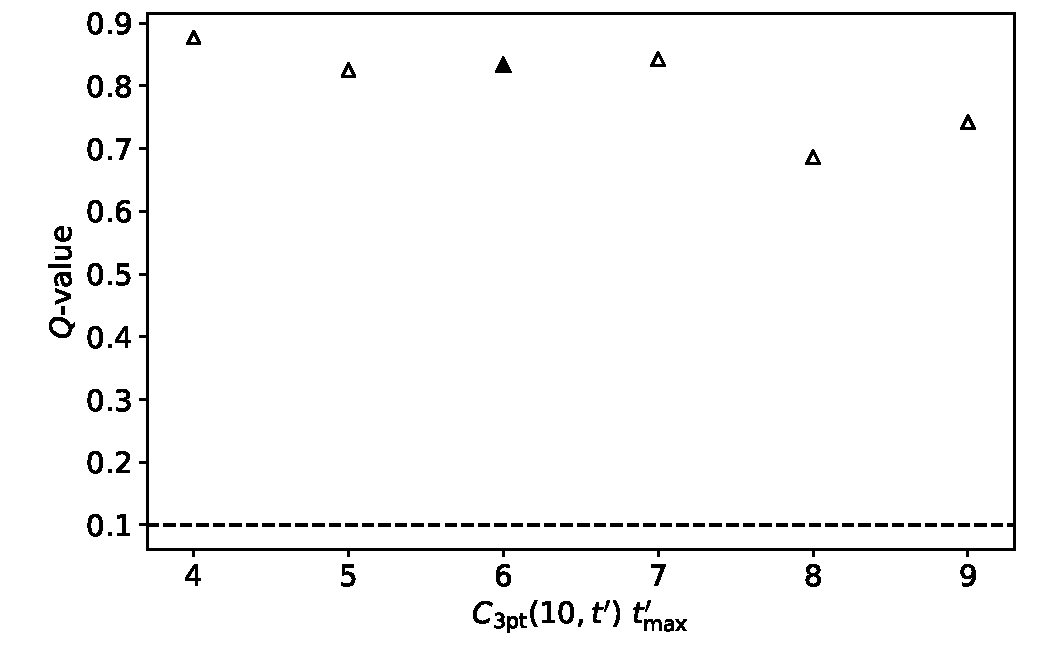
\includegraphics[width=0.49\textwidth]{plots/figures/3296_gV10_tmax_Q.pdf}
		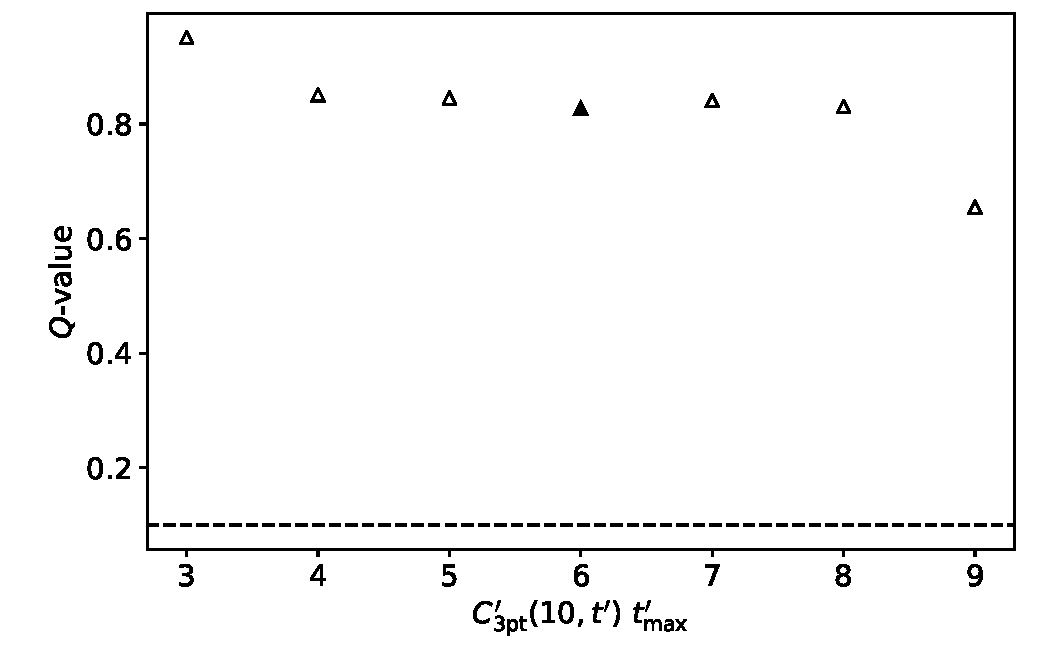
\includegraphics[width=0.49\textwidth]{plots/figures/3296_dgV10_tmax_Q.pdf}
		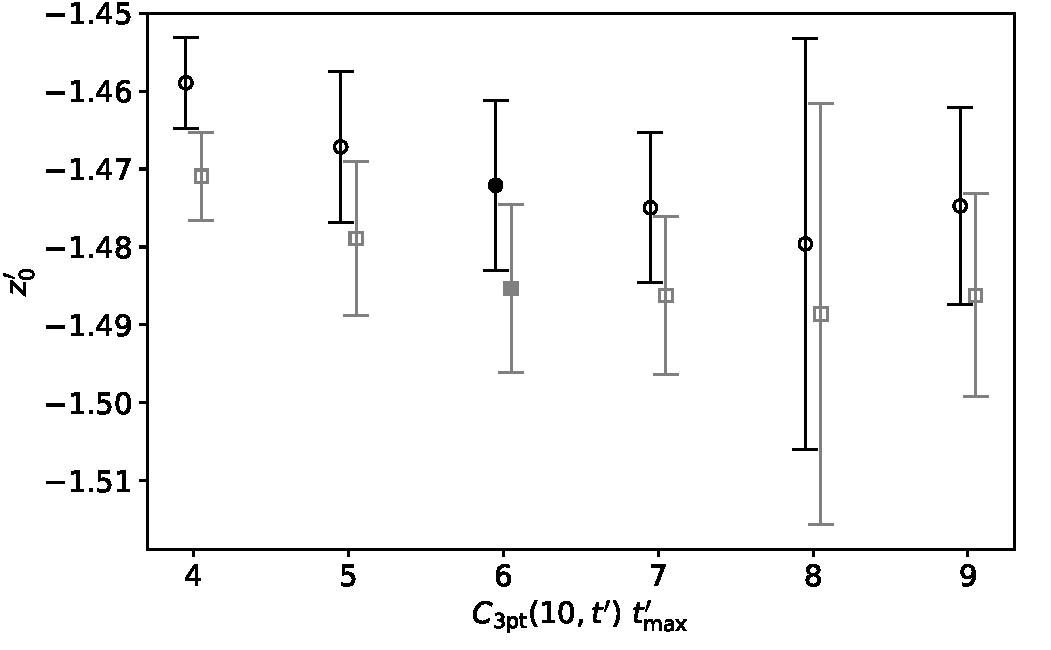
\includegraphics[width=0.49\textwidth]{plots/figures/3296_gV10_tmax_dZ0.pdf}
		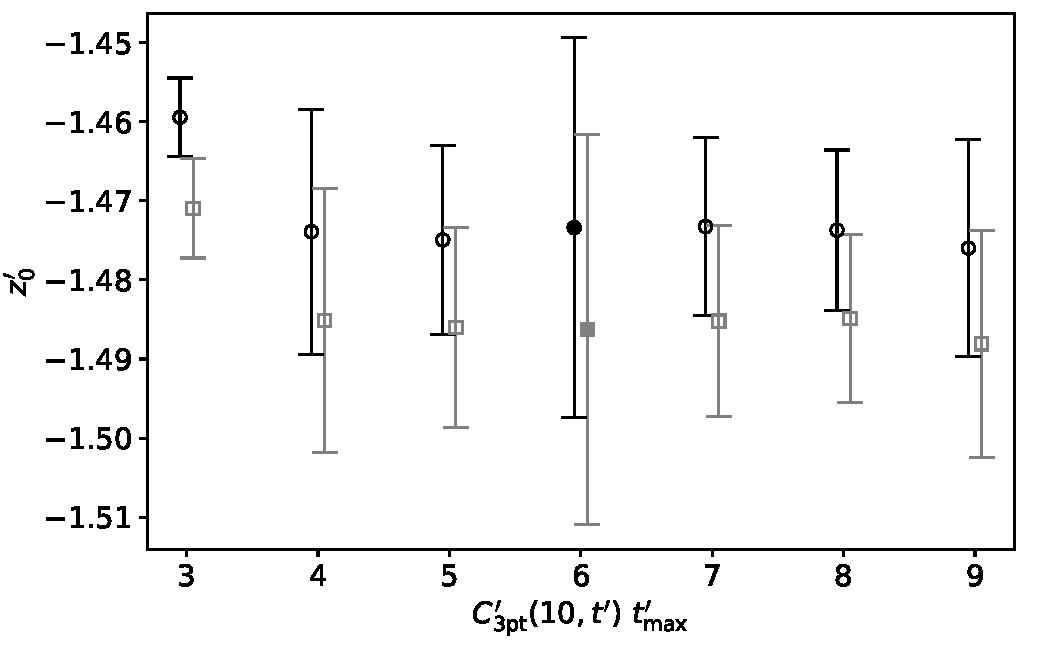
\includegraphics[width=0.49\textwidth]{plots/figures/3296_dgV10_tmax_dZ0.pdf}
		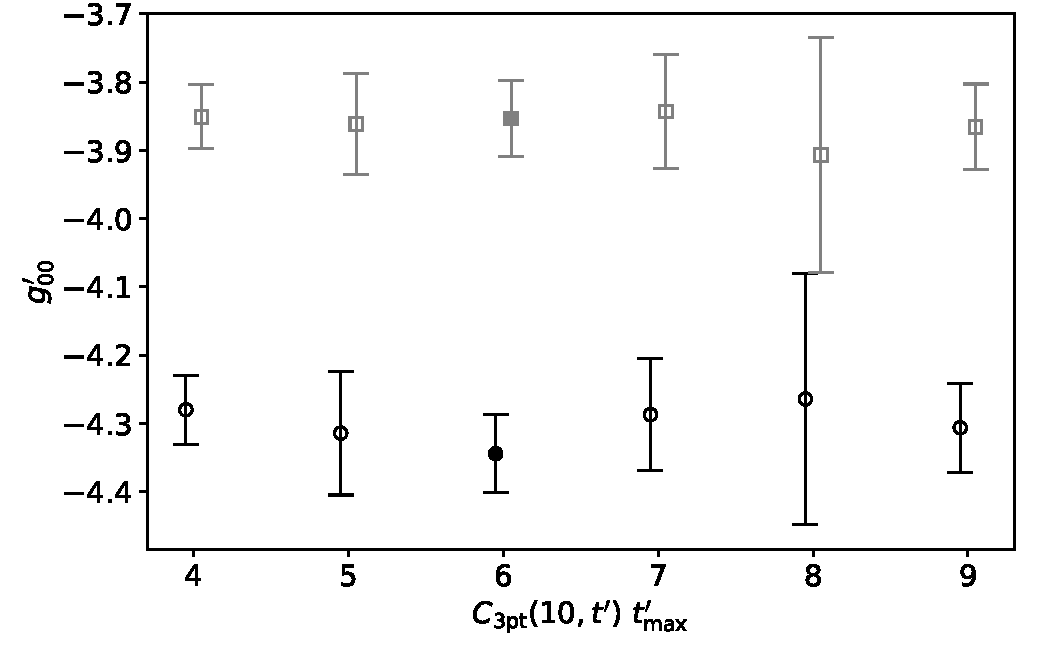
\includegraphics[width=0.49\textwidth]{plots/figures/3296_gV10_tmax_dgV.pdf}
		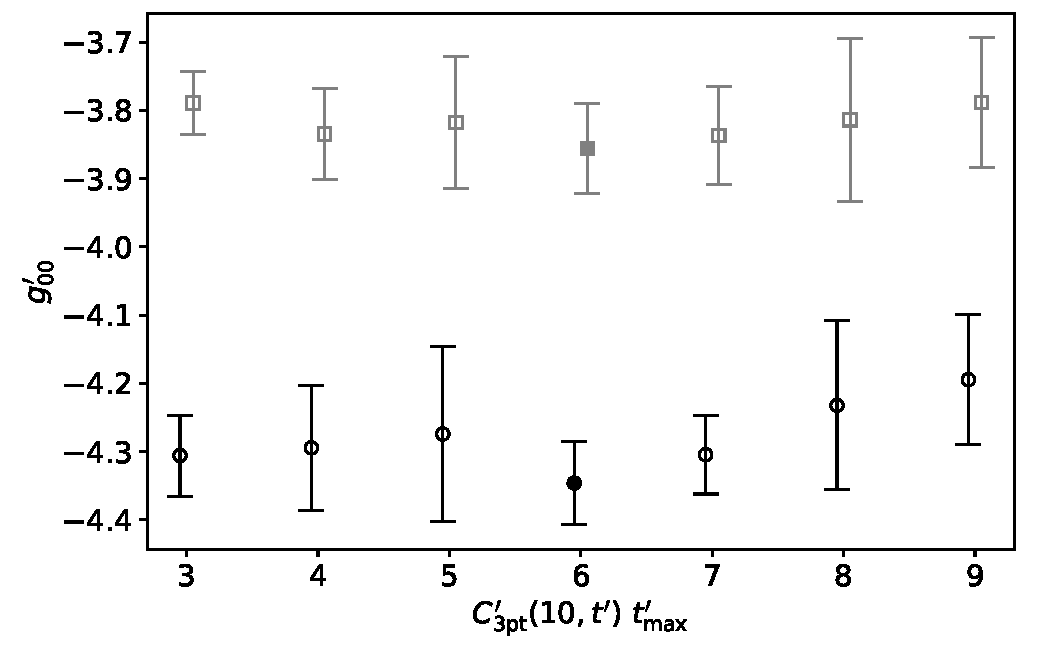
\includegraphics[width=0.49\textwidth]{plots/figures/3296_dgV10_tmax_dgV.pdf}
		\caption{
			Fit sensitivity to variations of $C_{\mathrm{3pt}}(10,t^\prime)$ and $C^\prime_{\mathrm{3pt}}(10,t^\prime)$ fit regions. For $C_{\mathrm{3pt}}$, the data is removed symmetrically around the mid-point. Analogous to Fig.~\ref{fig:stability_c2pt}.}
		\label{fig:stability_c3pt10}
}\end{figure*}
%\end{comment}

\end{document}
